\documentclass[10pt,leqno]{article}
\usepackage{dynkin-diagrams}
\usepackage{authblk}
\usepackage{amssymb}
\usepackage{amsrefs}
\usepackage{verbatim}
\usepackage{array}

\newcommand{\remind}[1]{{\bf ** #1 **}}
%\usepackage{showlabels}
%\usepackage{pifont}
\usepackage{tikz}
\newcommand*\circled[1]{\tikz[baseline=(char.base)]{
            \node[shape=circle,draw,inner sep=2pt] (char) {#1};}}
\usepackage{rotating}
\usepackage{amsmath}
\usepackage{tabularx}
\usepackage{caption}
\usepackage{theorem}
\usepackage[matrix,tips,frame,color,line,poly]{xy}
%\usepackage[dvips]{graphicx}

\renewcommand{\labelenumi}{(\arabic{enumi})}

\newtheorem{theorem}[equation]{Theorem}
\newtheorem{corollary}[equation]{Corollary}
\newtheorem{definition}[equation]{Definition}
\newtheorem{lemma}[equation]{Lemma}
\newtheorem{desideratum}[equation]{Desideratum}
\newtheorem{conjecture}[equation]{Conjecture}
\newtheorem{proposition}[equation]{Proposition}
\newtheorem{remark}[equation]{Remark}
{\theorembodyfont{\rmfamily}
\newtheorem{theoremplain}[equation]{Theorem}
\newtheorem{remarkplain}[equation]{Remark}
\newtheorem{editorialremarkplain}[equation]{Editorial Remark}
\newtheorem{exampleplain}[equation]{Example}
\newtheorem{corollaryplain}[equation]{Corollary}
}
\newcommand{\qed}{\hfill $\square$ \medskip}
\newenvironment{proof}[1][Proof]{\noindent\textbf{#1.} }{\qed}
\newcommand\exact[3]{1\rightarrow #1\rightarrow #2\rightarrow #3\rightarrow1}
\newcommand{\Aut}{\text{Aut}}
\newcommand{\sgn}{\text{sgn}}
\newcommand{\sig}{\text{sig}}
\newcommand{\hodge}{\text{hodge}}
\newcommand{\triv}{\text{triv}}
\newcommand{\diag}{\text{diag}}
\newcommand{\codim}{\text{codim}}
\newcommand{\gr}{\text{gr}}
\newcommand{\Out}{\text{Out}}
\newcommand{\Int}{\text{Int}}
\renewcommand{\int}{\text{int}}
\newcommand{\h}{\mathcal H}
\newcommand{\D}{\mathcal D}
\renewcommand{\j}{\mathcal J}
\newcommand{\Hreg}{H_{\text{reg}}}
\newcommand{\reg}{\text{reg}}
\newcommand{\Hom}{\text{Hom}}
\newcommand{\cox}{\text{Cox}}
\newcommand{\mult}{\text{mult}}
\newcommand{\Ind}{\text{Ind}}
\newcommand{\End}{\text{End}}
\newcommand{\PS}{\text{PS}}
\newcommand{\ad}{\text{ad}}
\newcommand{\Ad}{\text{Ad}}
\newcommand{\Lie}{\text{Lie}}
\newcommand{\Stab}{\text{Stab}}
\newcommand{\Norm}{\text{Norm}}
\newcommand{\Cent}{\text{Cent}}
\newcommand{\X}{\mathcal X}
\newcommand{\Y}{\mathcal Y}
\newcommand{\caZ}{\mathcal Z}
\newcommand{\caM}{\mathcal M}
\newcommand{\caI}{\mathcal I}
\newcommand{\I}{\mathcal I}
\renewcommand{\O}{\mathcal O}
%\renewcommand{\S}{\mathcal S}
\newcommand{\caN}{\mathcal N}
\newcommand{\caW}{\mathcal W}
\newcommand{\caP}{\mathcal P}
\newcommand{\caH}{\mathcal H}
\newcommand{\caPreg}{\mathcal P_{\text{reg}}}
\newcommand{\chPreg}{\ch P_{\text{reg}}}
\newcommand{\caT}{\mathcal T}
\newcommand{\caC}{\mathcal C}
\newcommand{\caA}{\mathcal A}
\newcommand{\tX}{\widetilde{\mathcal X}}
\newcommand{\tS}{\widetilde{\mathcal S}}
\newcommand{\tL}{\widetilde{\mathcal L}}
\newcommand{\tP}{\widetilde{\mathcal P}}
\newcommand{\tx}{\widetilde{x}}
\newcommand{\tphi}{\widetilde{\phi}}
\newcommand{\F}{\mathbb F}
\newcommand{\R}{\mathbb R}
\newcommand{\C}{\mathbb C}
\newcommand{\Z}{\mathbb Z}
\newcommand{\W}{\mathbb W}
\newcommand{\Ztwo}{\mathbb Z/2\Z}
\newcommand{\N}{\mathbb N}
\newcommand{\Q}{\mathbb Q}
\renewcommand{\F}{\mathbb F}
\newcommand{\E}{\mathcal E}
\newcommand{\caD}{\mathcal D}
\newcommand{\caS}{\mathcal S}
\newcommand{\caL}{\mathcal L}
\newcommand{\caB}{\mathcal B}
\newcommand{\chcaD}{\mathcal D^\vee}
\newcommand{\T}{\mathbb T}
\newcommand{\Gsc}{G_{\text{sc}}}
\newcommand{\Gad}{G_{\text{ad}}}
\renewcommand{\H}{\mathbb H}
{\renewcommand{\h}{\mathfrak h}}
\renewcommand{\q}{\mathfrak q}
\renewcommand{\u}{\mathfrak u}
\renewcommand{\a}{\mathfrak a}
\newcommand{\A}{\mathbb A}
\newcommand{\K}{\mathbb K}
\newcommand{\B}{\mathbb B}
\newcommand{\spint}{\widetilde{Spin}}
\newcommand{\tH}{\widetilde H}
\newcommand{\tG}{\widetilde G}
\newcommand{\tW}{\widetilde W}
\newcommand{\tK}{\widetilde K}
\newcommand{\tD}{\widetilde D}
\newcommand{\bD}{\overline D}
\newcommand{\bp}{\overline\Pi}
\newcommand{\tM}{\widetilde M}
\newcommand{\dual}[2]{^{#1}#2}
%\newcommand{\Ch}[1]{#1{\text{\large\v{}}}}
\newcommand{\ch}[1]{#1^\vee}
%\newcommand{\ch}[1]{{\text{\large\v{}}}#1}
\newcommand{\chG}{\ch{G}}
\newcommand{\chT}{\ch{T}}
\newcommand{\tildeint}{{\~{}\it{--integral}}\ }
\renewcommand{\L}[1]{^L#1}
\renewcommand{\sec}[1]{\section{#1}
\renewcommand{\theequation}{\thesection.\arabic{equation}}
  \setcounter{equation}{0}}
\newcommand{\subsec}[1]{\subsection{#1}
\renewcommand{\theequation}{\thesubsection.\arabic{equation}}}
\renewcommand{\t}{\mathfrak t}
\newcommand{\mi}{\medskip\noindent}
\newcommand{\si}{\smallskip\noindent}
\newcommand{\g}{\mathfrak g}
\newcommand{\GGamma}{G^\Gamma}
\newcommand{\GGammaG}{G^\Gamma\backslash G}
\newcommand{\chGGamma}{G^{\vee\Gamma}}
\newcommand{\WGamma}{W^\Gamma}
\newcommand{\weil}{W_\R}
\newcommand\inv{^{-1}}
\newcommand\bs{\backslash}
\newcommand\wt{\widetilde}
\newcommand\wh{\widehat}
\newcommand\fix[1]{{\noindent\bf#1}}
\newcommand\kgb{{\tt KGB}}
\newcommand{\Khat}{\widehat K}
\newcommand{\Wconj}{[W]}
\newcommand{\Weconj}{[{W^e}]}
\newcommand{\Gssconj}{[{G^\text{ss}}]}
\renewcommand{\ss}{\text{ss}}
\newcommand{\e}{\text{e}}
\newcommand{\Gss}{G^\ss}
\newcommand{\Wext}{\negthinspace\negthinspace\phantom{a}^\delta W}
\newcommand{\Text}{\negthinspace\negthinspace\phantom{a}^\delta T}
\newcommand{\Gext}{\negthinspace\negthinspace\phantom{a}^\delta G}
\newcommand{\Lext}{\negthinspace\negthinspace\phantom{a}^\delta L}
\newcommand{\Waff}{W_{\text{a}}}
\newcommand{\Waffe}{\wt W_{\text{a}}}
\newcommand{\Gdelta}{G^{\delta}}
\newcommand{\Daffine}{\wt D(G,\delta)}
\def\fh{\mathfrak h}
\def\fg{\mathfrak g}
\def\fc{\mathfrak c}
\def\fm{\mathfrak m}
\def\ft{\mathfrak t}
\def\fs{\mathfrak s}
\def\fb{\mathfrak b}
\def\fp{\mathfrak p}
\def\fl{\mathfrak l}
\def\fn{\mathfrak N}
\def\fA{\mathfrak A}
\def\fH{\mathfrak H}
\def\fP{\mathfrak P}
\def\fU{\mathfrak U}
\def\fu{\mathfrak u}
\def\fo{\mathfrak o}
\def\fS{\mathfrak S}

\def\ge{\geqslant}
\def\le{\leqslant}
\def\a{\alpha}
\def\b{\beta}
%\def\g{\gamma}
\def\G{\Gamma}
\def\d{\delta}
%\def\D{\Delta}
\def\L{\Lambda}
%\def\e{\epsilon}
\def\et{\eta}
\def\io{\iota}
\def\o{\omega}
\def\p{\pi}
\def\ph{\phi}
\def\ps{\psi}
%\def\r{\rho}
\def\s{\sigma}
\def\t{\tau}
\def\th{\theta}
\def\k{\kappa}
\def\l{\lambda}
\def\z{\zeta}
\def\v{\vartheta}
\def\x{\xi}
\def\i{^{-1}}
\newcommand{\twoAeven}{\phantom{}^2\negthinspace A_{2n}}
\newcommand{\twoAodd}{\phantom{}^2\negthinspace A_{2n+1}}
\newcommand{\twoD}{\phantom{}^2\negthinspace D_{n}}
\renewcommand{\sec}[1]{\section{#1}
\renewcommand{\theequation}{\thesection.\arabic{equation}}
  \setcounter{equation}{0}}
\font\temporary=manfnt
\def\dbend{{\temporary\char127}} % dangerous bend sign
% Danger, Will Robinson!
\def\danger{\begin{trivlist}\item[]\noindent%
\begingroup\hangindent=3pc\hangafter=-2%\clubpenalty=10000%
\def\par{\endgraf\endgroup}%
\hbox to0pt{\hskip-\hangindent\dbend\hfill}\ignorespaces}
\def\enddanger{\par\end{trivlist}}

\begin{document}

\author{Jeffrey Adams}
\author{Xuhua He}
\author{Sian Nie}
\affil{Department of Mathematics, University of Maryland, jda@math.umd.edu}
\affil{Department of Mathematics, University of Maryland, xuhuahe@math.umd.edu}
\affil{Institute of Mathematics, Academy of Mathematics and Systems Science, Chinese Academy of Sciences, 100190, Beijing, China
  , niesian@amss.ac.cn}
\date{}                     %% if you don't need date to appear


\title{From conjugacy classes in  the Weyl group to semisimple conjugacy classes}


\maketitle

\let\thefootnote\relax\footnotetext{X.~H.~was partially supported by
  NSF DMS-1801352. S.N. is supported in part by QYZDB-SSW-SYS007 and
  NSFC grant (No. 11621061).}

\let\thefootnote\relax\footnotetext{{\bf Keywords}: algebraic groups,
  Weyl groups, elliptic conjugacy classes, semisimple conjugacy
  classes}

\let\thefootnote\relax\footnotetext{{\bf 2010 Mathematics Subject
    Classification}: Primary 20G07, Secondary: 20F55, 20E45}

\noindent{\bf Abstract:} Suppose $G$ is a connected complex semisimple group
and $W$ is its Weyl group. The lifting of an element of $W$ to $G$ is
semisimple. This induces a well-defined map from the set of elliptic
conjugacy classes of $W$ to the set of semisimple conjugacy classes of
$G$. In this paper, we give a uniform algorithm to compute this
map. We also consider the twisted case.

\begin{center}

  
  \large \emph{To Bert Kostant with admiration}
  \end{center}

\sec{Introduction}

Let $G$ be a connected complex semisimple group.
Choose a Cartan subgroup $T\subset G$, let $N(T)$ be the normalizer of $T$ in $G$,
and let $W=N(T)/T$ be the Weyl group.
We have the exact sequence
\begin{equation}
\label{e:exactW}
1\rightarrow T\rightarrow N(T)\overset p\rightarrow W\rightarrow 1.
\end{equation}
In \cite{AH} we considered the question of whether this sequence splits,
and more generally if $w\in W$, what can be said about the order of $p\inv(w)$.
Here we consider a related problem.

Let $\Wconj$ be the set of conjugacy classes in $W$. Let $\Gss$ be the
semisimple elements of $G$, and $\Gssconj$ the set of semisimple
conjugacy classes. We have $N(T)\subset \Gss$. For $w\in W$ write $[w]$ for the $W$-conjugacy
class of $w\in W$. Similarly for $g\in \Gss$ let $[g]$ be the
$G$-conjugacy class of $g$.

Suppose $w\in W$ and $n(w)\in p\inv(w)\in N(T)$. For general $w$ there
are many choices of $n(w)$, even up to conjugacy.  However in an
important special case the choice of $n(w)$ is unique up to
conjugation. We say $w\in W$ is {\it elliptic} if it has no nontrivial fixed
vectors in the reflection representation.  It is well known that if
$w$ is elliptic then any two elements of $p\inv(w)\subset N(T)$ are
$T$-conjugate (see Lemma \ref{l:conjugate}). \remind{As $n(w)$ is used in section 5 as Tits lifting, it is better to change to a different symbol here}

\begin{definition}
\label{d:basic}
Suppose $w\in W$ is elliptic.
Choose $n(w)\in p\inv(w)\subset N(T)$, and define
$$
\Psi: \Weconj\rightarrow\Gssconj: [w]\rightarrow [n(w)].
$$
This map is well defined on the level of conjugacy classes by Lemma \ref{l:conjugate}.
\end{definition}

This map has been studied by many people, including Reeder
\cite{reeder_torsion} and Gross-Levy-Reeder-Yu \cite{rgly}, for
applications to representations of $p$-adic groups and number theory.
Some tables for simply laced groups, obtained by case-by-case
calculations are in Bouwknegt \cite{bouwknegt}.  Our main result is a
uniform algorithm to compute this map. We give this algorithm in the
next section, after first discussing the twisted case. We use the
algorithm to compute complete tables for the (twisted and untwisted) exceptional
groups.

\subsec{The twisted case}
\label{s:twisted}

A pinning is a triple $(G,T,\{X_\alpha\mid \alpha\in\Pi\})$,
where $\Pi$ is a set of simple roots of $T$ in $G$, and for each
$\alpha\in\Pi$, $X_\alpha$ is an $\alpha$-weight vector.  
We say an automorphism of $G$ is {\it distinguished} if it preserves some pinning.  An
inner automorphism is distinguished if and only if it is trivial as
any two pinnings are conjugate by a unique inner automorphism,
and the
outer automorphism group of $G$ is isomorphic to the group of
automorphisms of a pinning.

Suppose $\Pi$ is a fixed set of simple roots, and
$(G,T,\{X_\alpha\mid\alpha\in\Pi\})$ is a pinning.
Suppose $\delta$ is an automorphism of $G$, preserving
the pinning.
Then $\delta$ induces an
automorphism of $W$, which we also denote by $\delta$. We define
$$
\Gext=G \rtimes\langle\delta\rangle, \quad \Wext=W\rtimes\langle\delta\rangle.
$$
Then $\Wext\simeq \Norm_{\Gext}(T)/T$, and we write $p:\Norm_{\Gext}(T)\rightarrow \Wext$.

Let $\Delta=\Delta(T,G)$ be the root system, and
$V=\Q\langle\Delta\rangle$. This is a representation of $\Wext$ which
we refer to as the reflection representation.  We say $y\in\Wext$ is
elliptic if it has no nontrivial fixed vectors in the reflection
representation.  Write $[y]$ for the $\Wext$-conjugacy class of
$y$. We consider elements $y\in W\delta$, and write $[(W\delta)^e]$
for the $\Wext$-conjugacy classes of elliptic elements in $W\delta$.

From the identity $\delta\inv(\delta w)\delta=w(\delta w)w\inv$ it
follows that two elements of $W\delta$ are $\Wext$-conjugate if and
only if they are $W$-conjugate.

We say an element $y$ of $\Gext$ is {\it semisimple} if $\Ad(y)$ is
semisimple.  Write $[y]$ for the $\Gext$-conjugacy class of
$y\in \Gext$. We consider elements $y\in G\delta$, and write
$[(G\delta)^{\ss}]$ for the $G$-conjugacy classes of semisimple
elements in $G\delta$.  As in the case of $\Wext$, two elements of
$G\delta$ are $G$-conjugate if and only if they are $\Gext$-conjugate.

\begin{lemma}
\label{l:conjugate}
Suppose $w\in W\delta$ is elliptic.
Then any two
elements of $p\inv(w)\subset\Norm_{\Gext}(T)$ are $T$-conjugate.
\end{lemma}

\begin{proof}
Suppose $g\in p\inv(w)\subset \Norm_G(T)\delta$. 
Then for $t\in T$
$$
tgt\inv=tw(t\inv)g.
$$
Since $w$ is elliptic the map $t\rightarrow tw(t\inv)$ has finite
kernel, so is surjective.

Now suppose $g_1,g_2\in p\inv(w)$.
Since $w\in W\delta$, $g_1,g_2\in G\delta$. Write $g_1=h_1\delta,g_2=h_2\delta$ with $h_1,h_2\in G$.
By the previous discussion choose $t$ so that $tw(t\inv)=h_2h_1\inv$. Then $tg_1t\inv=g_2$.
\end{proof}

\begin{definition}
 \label{d:basictwisted}
Suppose $w\in W\delta$ is elliptic.
Choose $n(w)\in p\inv(w)\subset \Norm_G(T)\delta$, and define
$$
\Psi: [(W\delta)^\e]\rightarrow[(G\delta)^{\ss}]: [w]\rightarrow [n(w)].
$$
This map is well defined on the level of conjugacy classes by Lemma \ref{l:conjugate}.
\end{definition}

If $w\in W\delta$ is not elliptic then the lifts $n(w)$ are not all $G$-conjugate. Nevertheless
by realizing $w$ as an elliptic element in a Levi subgroup one can define a canonical map
from $[(W\delta)^\e]$ to $[(G\delta)^{\ss}]$. See Section \ref{s:nonelliptic}.

We've stated the result over $\C$. The algorithm applies over any
algebraically closed field of characteristic $0$, and in general with
a weak restriction on the characteristic. See Remark
\ref{r:otherfield}.

The tables in Section \ref{s:tables} were calculated using the
{\it atlas of Lie groups and representations} software \cite{atlas_software} (see the file {\tt weyltosemisimple.at}).

The authors thank Tom Haines for numerous helpful discussions.

\sec{The Algorithm}
\label{const}

Assume $G$ is a semisimple reductive group defined over $\C$, and
$\delta$ is an automorphism of $G$ of finite order. We fix a pinning
$(G,T,\{X_\alpha\mid\alpha\in\pi\})$, and we may assume $\delta$
preserves this pinning.  Other notation is as in Section \ref{s:twisted}.

Suppose $w\in \Wext$. Let
\begin{subequations}
\renewcommand{\theequation}{\theparentequation)(\alph{equation}}
\label{e:algorithm}
\begin{equation}
\Gamma_w=\{0\le\theta\le\pi\mid\text{such that } e^{i\theta}\text{ is an eigenvalue of $w$\text{ on }}V_\C.\}
\end{equation}
Write
\begin{equation}
\label{e:thetas}
\Gamma_w=\{\theta_1,\theta_2,\dots,\theta_k\}\text{ with }\theta_1<\theta_2<\dots<\theta_k.
\end{equation}
For $\theta\in \Gamma_w$ let
\begin{equation}
V(w,\theta)=\{v\in V_\R\mid w(v)+w\inv(v)=2\cos(\theta)v\}.
\end{equation}
Then $V(w,\theta)_\C$ is the direct sum of the eigenspaces of
$w$ on $V_\C$ with eigenvalue $e^{\pm i\theta}$.

For $1 \le i \le k$ set
$$
F_i=\sum_{j=1}^i V(w,\theta_j)
$$
and set $F_0=0,\theta_0=0$. We have a filtration
\begin{equation}
\label{e:F_k}
0=F_0\subsetneqq F_1\dots \subsetneqq \dots\subsetneqq F_{k}=V
\end{equation}
with strict containments. For $0 \le i \le k$, set
\begin{equation}
\Delta_i=\{\alpha\in\Delta\mid \langle\alpha,F_i\rangle=0\}.
\end{equation}
Then each $\Delta_i$ is a root system, and set
\begin{equation}
W_i=W(\Delta_i).
\end{equation}
Thus we have
\begin{equation}
  \label{e:levis}
  \begin{aligned}
\Delta&=\Delta_0\supseteq \Delta_1\supseteq \dots\supseteq \Delta_k=\emptyset,\\
W&=W_0\supseteq W_1\supseteq \dots\supseteq W_k=\{1\}.\\
\end{aligned}
\end{equation}

After conjugating by $W$ we assume furthermore that all the $\Delta_i$ are
standard, i.e., the corresponding Levi subgroups are standard Levi
subgroups \cite{he_nie_minimal_finite}*{Lemma 5.1}).

For each $i$ set
\begin{equation}
\begin{aligned}
\Delta^+_i&=\Delta^+\cap \Delta_i,\\
\ch\rho_i&=\frac12\sum_{\alpha\in\Delta_i^+}\ch\alpha.
\end{aligned}
\end{equation}
We define rational coweights
$\{\ch\lambda_0,\dots, \ch\lambda_{k}\}$ by downward induction.
Set $\ch\lambda_k=0$, and for $0\le i\le k-1$ define
\begin{equation}
\begin{aligned}
\ch\lambda_{i}=\frac{d(\theta_{i+1}-\theta_{i})}{2\pi}\ch\rho_i+\overline{\ch\lambda_{i+1}},
\end{aligned}
\end{equation}
where $d$ is the order of $w$, $\overline{\ch\lambda_{i+1}}$ is the element in the $W_i$-orbit of $\ch\lambda_{i+1}$ which is dominant for $\Delta^+_i$.
\end{subequations}

\begin{theorem}
\label{t:main}
Suppose $w\in W\delta$ is of order $d$. Construct $\ch\lambda_0$ by the algorithm. Then
some lift $n(w)$ of $w$ is $G$-conjugate to $\exp(2\pi i\ch\lambda_0/d)\delta$.

In particular if $w\in (W\delta)^e$ then 
\begin{equation}
  \label{e:main}
  \Psi([w])=[\exp(2\pi i\ch\lambda_0/d)\delta].
\end{equation}
\end{theorem}

\begin{remarkplain}
\label{r:full}
The algorithm  uses the full sequence $(\th_1, \ldots, \th_k)$.
One may replace the full sequence by any subsequence that is
admissible in the sense of \cite{he_nie_minimal_finite}*{subsection
  5.2}.  The proof of the Theorem applies with no change in this
generality. The element $\exp(2\pi i\ch\lambda_0/d)\delta \in \Gext$ is
obtained from an admissible subsequence of $(\th_1, \ldots, \th_k)$
is, in general, different from the element obtained here using the
full sequence. However by the Theorem these elements are all
conjugate. %See example \ref{eg:regular}.
\end{remarkplain}

We will use the following conjugacy result\footnote{We thank Dipendra Prasad for bringing this result to our attention.}.

\begin{proposition}
Suppose $G$ is a finite group all of whose characters are defined over $\Q$. 
Suppose $g\in G$ has order $d$. If $(d,k)=1$ then 
 $g^k$ is conjugate to $g$.
\end{proposition}

\medskip

\begin{proof}
Let $F=\Q(\zeta_d)$ where $\zeta_d$ is a primitive $d^{th}$ root of unity.
If $\pi$ is a representation of $W$, with character $\theta_\pi$, then
$$
\theta_\pi(g)=\sum_{i=1}^r z_i,
$$
where each $z_i$ is a $d^{th}$ root of unity in $F$. Then
$$
\theta_\pi(g^k)=\sum_{i=1}^r z_i^k.
$$
Since $(k,d)=1$ the map $\zeta_d\rightarrow \zeta_d^k$ induces an automorphism $\tau$ of
$F/\Q$. By assumption  $\sum_i z_i\in \Q$, so
$$
\theta_\pi(g^k)=\sum_i z_i^k=\sum_i \tau(z_i)=\tau(\sum z_i)=\sum z_i=\theta_\pi(g).
$$
Since the characters separate conjugacy classes this implies $g$ is conjugate to $g^k$.

\end{proof}

We need a slight generalization of this.

\begin{proposition}
  \label{p:g^k}
Suppose $G$ is as in the previous Proposition, and  $\delta$
is an automorphism of $G$ of finite order. 
Let $\Gext=G\rtimes\langle\delta\rangle$. Suppose
$g\in G\delta\subset \Gext$ has order $d$.
Suppose $(k,d)=1$ and $g^k$ is also contained in $G\delta$. 
Then $g^k$ is conjugate to $g$.
\end{proposition}

Recall (Section \ref{s:twisted}) the statements with $G$-conjugacy or
$\Gext$-conjugacy are equivalent.

\begin{proof}
  Let $m$ be the order of $\delta$. By Clifford theory the characters of $\Gext$ are defined over
  $\Q(\zeta_m)$ where $\zeta_m$ is a primitive $m^{th}$ root of $1$.
  Replace $\Q$ with $E=\Q(\zeta_m)$ in the proof of the previous
  Proposition, and consider the field $E(\zeta_d)$. 
  The condition $g^k\in G\delta$ implies $k=1\pmod m$, so $\zeta_m^k=\zeta_m$ and 
  the map $\zeta_d\rightarrow \zeta_d^k$ induces an automorphism of $E(\zeta_d)/E$.
The  rest of the proof goes through with minor changes.
\end{proof}

\begin{remarkplain}
\label{r:otherfield}
Suppose $F$ is an algebraically closed field and the order of $\Wext$ is invertible in $F$.
Then all of the elements of $\Norm_{\Gext}(T)$ are semisimple
and a version of Theorem \ref{t:main} holds in this setting. The only issue is to make
sense of the right hand side of \eqref{e:main} over $F$. 

Suppose $\ch\lambda_0$ is constructed as in the algorithm. Choose $m\in\Z$ so that $m\ch\lambda_0\in X_*$,
and choose a primitive $dm^{th}$ root of unity $\zeta_{dm}\in F$. Then
$$
\Psi([w])=[\delta (m\ch\lambda_0)(\zeta_{dm})]
$$
where we view $m\ch\lambda_0$ as a one-parameter subgroup
corresponding to $m\ch\lambda_0:F^\times\rightarrow T(F)$. By
Proposition \ref{p:g^k} this is independent of the choices of $m$ and
$\zeta_{dm}$.

\end{remarkplain}


\sec{Digression on  good elements}
\label{s:digression}

The algorithm in Section \ref{const} is  motivated in part by
the construction of the good elements in a given conjugacy class of
$\Wext$. In this section, we discuss this
construction.

The good elements in $W$ were introduced by Geck and Michel in
\cite{geck_michel_good} and the notion was generalized to $\Wext$ by Geck, Kim and
Pfeiffer in \cite{gkp}.

Let $B^+$ be the braid monoid associated with $(W,S)$. Then there is a
canonical injection $j:W\longrightarrow B^+$ identifying the
generators of $W$ with the generators of $B^+$ and
satisfying $j(w_1w_2)=j(w_1)j(w_2)$ for $w_1,w_2\in W$ whenever
$\ell(w_1w_2)=\ell(w_1)+\ell(w_2)$.

Now the automorphism $\delta$ induces an automorphism of $B^+$, which
is still denoted by $\delta$. Set ${}^{\delta} B^+=B^+ \rtimes
\langle\delta\rangle$. Then $j$ extends in a canonical way to an
injection $\Wext \to {}^{\delta} B^+$, which we still denote by
$j$. We will simply write $\underline w$ for $j(w)$.

By definition, $w \in \Wext$ is a {\it good element} if there exists a
strictly decreasing sequence $\Pi_0 \supsetneq \Pi_1 \supsetneq \cdots
\supsetneq \Pi_l$ of subsets of $\Pi$ and even positive integers
$d_0,\cdots,d_l$ such
that $${\underline{w}}^d=\underline{w_0}^{d_0}\cdots\underline{w_l}^{d_l}.$$
Here $d$ is the order of $w$ and $w_i$ is the longest element of the
parabolic subgroup of $W$ generated by $\Pi_i$.

It was proved in \cite{geck_michel_good}, \cite{gkp} and \cite{he_minimal_length_double_cosets} that for any
conjugacy class of $\underline W$, there exists a good minimal length
element. In \cite{he_nie_minimal_finite}, the second and third-named authors
gave a general proof, which also provides an explicit construction of good
minimal length elements.

Now we recall the construction in \cite{he_nie_minimal_finite}.
Let $F_0,\dots, F_k$ be as in \eqref{e:F_k}.

Let $\caA$ be a Weyl chamber and for $0 \le i < k$, let $\caC_i(\caA)$
be the connected component of $V-\cup_{H_\a; F_i \subset H_\a}H$
containing $\caA$. We say $\caA$ is in {\it good position} with
respect to $w$ if for any $i$, the closure $\overline{\caC_i(\caA)}$
contains some regular point of $F_{i+1}$.

By \cite{he_nie_minimal_finite}*{Lemma 5.1}, there exists some Weyl chamber $\caA$ that is
in good position with respect to any given $w$. By definition, for any
$x \in W$, the Weyl chamber $x(\caA)$ is in good position with respect
to $x w x^{-1}$. In particular, for any conjugacy class of $\Wext$,
there exists an element $w$ such that the dominant chamber is in good
position with respect to $w$. In this case, $\Delta_i$ is the root system
of the standard Levi subgroup of $G$ associated to the subset
$\Pi_i:=\Pi \cap \Delta_i$ of simple roots and $W_i=W_{F_i}$ is a standard
parabolic subgroup of $W$ for any $i$. We denote by $W^{\Pi_i}$ (resp. ${}^{\Pi_i} W$) the
set of minimal length representatives in $W/W_i$ (resp. in $W_i \backslash W$). We write ${}^{\Pi_1} W^{\Pi_2}$ for ${}^{\Pi_1} W \cap W^{\Pi_2}$. By \cite{he_nie_minimal_finite}*{Proposition
2.2}, we have the following good factorization of $w$.

\begin{proposition}\label{good-fac} Let $w \in W \d \subset
\Wext$. Suppose that the dominant chamber is in good position with
respect to $w$. Then $$w=\d x_1 x_2 \cdots x_k,$$ where for $1 \le i
\le k$, we have $x_i \in W_{i-1} \cap W^{\Pi_i}$ and $\d_i=\d x_1
\cdots x_{i}$ such that $\d_i (\Pi_i)=\Pi_i$.
\end{proposition}

The following result is proved in \cite{he_nie_minimal_finite}*{Theorem 5.3}.

\begin{theorem}
\label{t:braid}
Let $w \in \Wext$ such that the fundamental chamber is
in good position with $w$. Then we have the following equality in the
Braid monoid associated with $(W, S)$: $$\underline w^d=\underline
w_0^{d \theta_1/\pi} \underline w_1^{d (\theta_2-\theta_1)/\pi} \cdots
\underline w_{k-1}^{d (\theta_{k}-\theta_{k-1})/\pi},$$ where $d$ is
the order of $w$ in $\Wext$, $(\theta_1, \cdots,
\theta_k)$ is the sequence consisting of all the elements in $\G_{w}$
and $w_i$ is the maximal element in the standard parabolic subgroup
$W_i$.
\end{theorem}

\sec{The regular case}
\label{s:regular}

We first study the regular elliptic elements. 
A similar discussion is in \cite{reeder_torsion}*{Section 2.6}.

Following
\cite{springer_regular} we say an element $w \in {}^{\delta} W$ is {\it regular} if it has a
regular eigenvector. We say $w$ is {\it $d$-regular} if the corresponding eigenvalue has
order $d$ ($d$ turns out to be independent of the choice of regular eigenvector).
Following \cite{rgly} we say
element $w$ is {\it $\mathbb Z$-regular} if $\langle w\rangle$ acts freely
on $\Delta$. The following result is proved in \cite[Prop. 1]{rgly}, see also \cite{AH}*{Lemma 7.2}.

\begin{lemma} Suppose $w\in W\delta$ is $d$-regular.  Then
$o(w)=\text{lcm}(o(\delta),d)$.  The following conditions are
equivalent:
	\begin{enumerate}
		\item $d=o(w)$,
		\item $o(\delta)$ divides $d$,
		\item $w$ is $\mathbb Z$-regular.
	\end{enumerate}
\end{lemma}

In particular if $w$ is $\Z$-regular then it is $d$-regular for some $d$, and if $\delta=\text{id}$ the converse holds.
The converse does not hold in general. %:in type ${}^2 E_6$, the elements with characteristic polynomial $\Phi_6 \Phi_3^2$ are of order $6$ and are $3$-regular (see \cite{springer_regular}*{Table 8}), but not $\Z$-regular. (This is the only exception in a simple group.)

\begin{proposition}\label{regular} Suppose $w \in W\d$ is elliptic and
regular. Let $\theta \in \G_w$ such that $V(w, \theta)$ contains a
regular vector of $V$. Then $[n(w)]=[\exp(i \theta\rho^\vee)\delta]$.
\end{proposition}
\begin{remark}
The case where $w$ is $\mathbb Z$-regular is proved in \cite{rgly}*{Prop. 12}. 
\end{remark}

\begin{proof} Let $\zeta=\exp(i \theta)$ and let
$\t=\delta \exp(i \theta \rho^\vee)=\delta \rho^\vee(\zeta)$. Let $d,m$ be
the orders of $\zeta \in \mathbb C^\times$ and $\t$ respectively.
Let $\xi$ be a primitive $m$-th root of unity such that
$\zeta=\xi^{m/d}$. We set $\iota=\tau^d=\delta^d$. Let $\fg, \ft$ be
the Lie algebras of $G$ and $T$ respectively. We denote by
$\fg^\iota$ and $\ft^\iota$ the subalgebras of $\iota$-fixed points
of $\fg$ and $\ft$ respectively. Then $\fg^\iota$ is also a
semisimple Lie algebra and $\ft^\iota$ is a Cartan subalgebra of
$\fg^\iota$.

	The automorphism $\t$ gives a periodic grading: $\fg=\oplus_{i
\in \mathbb Z/m\mathbb Z} \fg_i$, where $\fg_i$ is the
$\xi^i$-eigenspace of $\fg$ for $\t$. Then we have $\fg^\iota =
\oplus_{i \in \mathbb Z / d\mathbb Z} \fg^\iota_i$, where
$\fg^\iota_i=\fg_{im/d}$ is the $\zeta^i$-eigenspace for $\t$. This is
an $N$-regular periodic grading of ${\fg}^{\iota}$, see
\cite{panyushev}*{Section 3}.
	
Let $\fc' \subseteq \fg^\iota_1$ be a Cartan subspace. By the
construction in \cite{rgly}*{Subsection 3.1}, there is a $\t$-stable
Cartan subalgebra $\fs'$ of $\fg^\iota$ containing $\fc'$. Let $\fs$
be the centralizer of $\fs'$ in $\fg$. As $\fs'$ is conjugate to
$\ft^\iota$, $\fs$ is also a Cartan subalgebra of $\fg$ fixed by
$\t$. Let $g \in G$ such that $\ft=\Ad(g) \fs$, and set $\varepsilon=g
\t g\i$. Then $\varepsilon \in G \d$ fixes $\ft$ and lies in $N \d$,
where $N$ is the normalizer of $T$ in $G$. Let $\ft(n(w), \z)$ and
$\ft(\varepsilon, \z)$ be the $\z$-eigenspaces of $\ft$ for $n(w)$ and
$\varepsilon$ respectively. Thanks to
\cite{springer_regular}*{Theorem 6.4 (iv)} and
the ellipticity of $w$, to show $n(w)$ and $\varepsilon$ are conjugate,
it suffices to show $$\dim \ft(n(w), \z)= \dim \ft(\varepsilon, \z).$$
Notice that $\ft(\varepsilon, \z)=\Ad(g) \fc'$.
	
	Let $v \in V(w, \theta)$ be a regular point. We may assume
that $v$ is (strictly) dominant. Since $w^d(v)=v$ and $v$ is strictly
dominant, one has $w^d=\d^d=\iota$ and hence $w \in W^\iota \d$, where
$W^\iota$ is the subgroup of $\iota$-fixed points of $W$. Notice that
$\ft(n(w), \z)=\ft^\iota(n(w), \z)$ and that $W^\iota$ is the Weyl group
of $\ft^\iota$ in $\fg^\iota$, where $\ft^\iota(n(w), \z)$ is the
$\z$-eigenspace of $\ft^\iota$ for $n(w)$. Then
\cite{springer_regular}*{Theorem 6.4 (ii)} says $$\dim \ft(n(w), \z) = \dim \ft^\iota(n(w), \z)=
a(d, \d),$$ where $a(d, \d)$ is defined in
\cite{springer_regular}*{Section 6} with
respect to $W^\iota$ and $\d$.
	
	On the other hand, applying \cite{panyushev}*{Theorem 3.3 (v)} to the
$N$-regular periodic grading $\fg^\iota = \oplus_{i \in \mathbb Z /
d\mathbb Z} \fg^\iota_i$, one deduces that $$\dim \ft(\varepsilon, \z)
= \dim \fc' = a(d, \d).$$ The proof is finished.
\end{proof}

\begin{corollary}
Suppose $w\in W\delta$ is elliptic and $d$-regular. Then
$$
[n(w)]=[\exp(2\pi i\ch\rho/d)\delta].
$$
\end{corollary}

This follows from the fact that $V(w,2\pi/d)$ contains a regular vector.

\begin{comment}
This follows from the fact that the sequence consisting of a singleton
$(2\pi/d)$ is admissible in the sense of
\cite{he_nie_minimal_finite}*{\S 5.2}, see Remark
\ref{r:full}.
\end{comment}

\begin{comment}
\subsection{Example}\label{eg:regular}
Let $W$ be of type $E_6$ and let $\d$ be the unique nontrivial
automorphism of $(W, \Pi)$. Up to $W$-conjugation, there is a unique
3-regular element $w \in W \d$ of order 6, whose characteristic
polynomial is $\Phi_6 \Phi_3^2$, see \cite{springer_regular}*{Table
  8}. Note that $w$ is regular, but not $\mathbb Z$-regular. Moreover,
$\G_w=\{2\pi/6, 2\pi/3\}$ and the associated filtration is
$0 \subsetneqq F_1 = V(w,\frac{2\pi}{6}) \subsetneqq V$. Let
$\Delta_1 = \{\a \in \Delta; \langle\alpha, F_1\rangle = 0\}$.

Notice that $w^3 \in W\d$ is 1-regular and $\dim V^{w^3}=4$. On the other hand, $\d$ is also 1-regular and $\dim V^\d=4$. So $w^3$ is conjugate to $\d$ by
\cite{springer_regular}*{Theorem 6.4 (iv)}. In particular, $V(w, \frac{2\pi}{6})$ is conjugate to  $V(\d, \pi)$.

The simple roots of $E_6$ are labeled as follows.

$$
\begin{dynkinDiagram}[Kac,label,ordering=Bourbaki,root radius=.12cm, edge  length=1.0cm]{E}{6}
\end{dynkinDiagram}
$$
\medskip

The $\d$-orbits on $\Pi$ are $\{1, 6\}$, $\{3, 5\}$, $\{2\}$ and $\{4\}$. So $V(\d, \pi)$ is spanned by $(1, 0, 0, 0, 0, -1)$ and $(0, 0, 1, 0, -1, 0)$. Here $\mu=(\mu_1, \dots, \mu_6) \in \mathbb Z^6$ stands for the vector $\sum_{i=1}^6 \mu_i \a_i^\vee \in \mathbb Z \Delta^\vee$. One checks that the root system $\Delta' = \{\a \in \Delta; \langle \a, V(\d, \pi)\rangle=0\}$ is of type $D_4$, which is conjugate to the root system $\Delta''$ spanned by $\{2, 3, 4, 5\} \subseteq \Pi$. Up to $W$-conjugation, we can assume $\Delta_1 = \Delta''$.

Now one computes that $\l_1^\vee = \rho_1^\vee=(0, 3, 3, 5, 3, 0)$ and its dominant conjugate is $\overline{\l_1^\vee}=(3, 5, 6, 9, 6, 3)$. Note that $\rho^\vee=(8, 11, 15, 21, 15, 8)$. Then the full sequence gives
$$
t=\delta \exp(\frac{2\pi i}{6} \l_0)=\delta\exp(\frac{2\pi i}{6} (\rho^\vee + \overline{\l_1^\vee}))=\delta \exp(\frac{2\pi i}{6} (11, 16, 21, 30, 21, 11)).
$$
The partial sequence gives
$$
t'=\delta \exp(\frac{2\pi i}{3} \rho^\vee)=
\delta \exp(\frac{2\pi i}{6} (16, 22, 30, 42, 30, 16)).
$$
So $t \neq t'$. On the other hand, we have
\begin{gather*} t_1:=n(s_1 s_6) t n(s_1 s_6)^{-1} =\delta \exp(\frac{2\pi i}{6}(10, 16, 21, 30, 21, 10)); \\
t_2:=\a_3^\vee(-1) t_1 \a_3^\vee(-1)=\delta \exp(\frac{2\pi i}{6}(10, 16, 18, 30, 24, 10))=t'.
\end{gather*}
So $t$ is conjugate to $t'$.

\bigskip
\end{comment}

\sec{The inductive step}

\subsection{The element $\l_0^\vee$ is $\d$-stable}
Assume that the dominant chamber $\caC$ is in good position with
$w$. Let $w=\d x_1 x_2 \cdots x_k$ be the good factorization of $w$ as
in Proposition \ref{good-fac}. We first show that the coweight
$\l_0^\vee$ we constructed in section \ref{const} is fixed by $\d$.

\begin{lemma} \label{dom}
	We have $\l_0^\vee =\delta (\l_0^\vee)$.
\end{lemma}
\begin{proof}

  Recall (Proposition \ref{good-fac})  $\d_i=\delta x_1 \cdots x_{i}$. We show by induction that
  $\d_{i}(\l^\vee_{i})=\l^\vee_{i}$ for $0 \le i \le k$. If $i=k$,
  then $\l_k^\vee = 0$ and the statement is obvious. Assume
  $\d_{i+1}(\l_{i+1}^\vee) = \l_{i+1}^\vee$ for some
  $0 \le i \le k-1$. We prove $\d_i(\l_i^\vee)=\l_i^\vee$. Since
  $\d_{i}(\Delta_i^+)=\Delta_i^+$, we
  have $$\d_{i}(\rho_i^\vee)=\rho_i^\vee.$$ Let $y_i \in W_i$ such
  that $\overline{\l_{i+1}^\vee} =
  y_i(\l_{i+1}^\vee)$. Then
  $$\overline{\l_{i+1}^\vee}=y_i \d_{i+1} y_i^{-1}
  (\overline{\l_{i+1}^\vee}) =y_i \d_i x_{i+1} y_i^{-1}
  (\overline{\l_{i+1}^\vee}).$$ Note that
  $y_i \d_i x_{i+1} y_i^{-1} \in W_i\delta_i$ and that
  $\overline{\l_{i+1}^\vee}$ is dominant for $\Delta_i^+$. Therefore,
  $\d_i$ fixes $\overline{\l_{i+1}^\vee}$ and hence also fixes
  $\l_i^\vee$ as desired.
\end{proof}

\subsection{The lifting $n(x)$}\label{setup}

We prove the main result using the induction argument for the triple $(\Delta, \d, w)$ with $w$ an element in $W(\Delta) \d$. 

We may regard $\delta\circ\Ad(x_1)$ as an automorphism of $W_1$ and of
the Levi subgroup $L_{\Pi_1}$ associated to $\Pi_1$. Then
$\d_1 x_2 \cdots x_k$ is an element of
$W_1 \rtimes \langle\d \circ \Ad(x_1)\rangle$. Thus by the inductive
hypothesis on $(\Delta_1, \d_1, w)$, we have that

(a) $n(w)$ is conjugate to $n(\d_1) \exp(\frac{2 \pi i \l^\vee_1}{d}) \in L_{\Pi_1} \rtimes \langle\d \circ \Ad(x_1)\rangle$.

In the next step, we would like to conjugate $n(\d_1)$ to an element
in $T \d$. Note that $\d_1$ is not an elliptic element of ${}^\d W$ in
general.  Hence the liftings of $\d_1$ are not all conjugate in
$G$. In particular, the Tits lifting of the elements in the conjugacy
class of $\d_1$ are not all conjugate in $G$. For the purpose of our
argument, we fix a set of lifts $n(x) \in N_G(T)$ for $x \in {}^\d W$
such that

(1) $n(s_\a)^2=\exp(\pi i \a^\vee)$ for $\a \in \Pi$;

(2) $n(x x') = n(x) n(x')$ if $\ell(x x') = \ell(x) + \ell(x')$.

We need a formula for the cycle defined by these lifts.

\begin{lemma} \label{factor}{\cite{ls}*{Lemma 2.1A}}
Given $x,y\in \Wext$ let
$$
\gamma^\vee=\sum_{\b \in \Delta^+ \cap y \i(\Delta^-) \cap y \i x \i (\Delta^+)} \b^\vee.
$$
Then
$$
n(x)n(y)=\exp(\pi i\gamma^\vee) n(xy)
$$
\end{lemma}


\begin{lemma} \label{average}
  Let $x \in W_0 \d$ and  $d \in \mathbb Z_{\ge 1}$ such that $x^d=1$. Let $v\in V$. Then the element $n(x)\exp(2 \pi i v)$ is conjugate to
  $n(x) \exp(\frac{2 \pi i}{d}\sum_{k=0}^{d-1} x^k(v))$ by an element in $T$.
\end{lemma}
\begin{proof}
Let
$$
r=\exp(\frac{2\pi i }{d}\sum_{k=0}^{d-1} k x^{-k}(v)).
$$
Then $r^{-1} n(x)\exp(2 \pi i v) r = n(x) \exp(2\pi i\frac{1}{d}\sum_{i=0}^{d-1} x^i(v))$ as desired.
\end{proof}

\subsection{Analysis of the element $n(\d_1)$}\label{5.3}

We first show that

\begin{lemma}
	Let $\Delta'=\{\a \in \Delta; \langle\a, V^{\d_1}\rangle=0\}$ and let $V'$ be the subspace of $V$ spanned by $\Delta'$. Then no roots in $\Delta'$ vanishes identically on $V(\d_1, \th_1)$.
\end{lemma}
\begin{proof}
	Let $\a \in \Delta'$. We have to show that $\langle\a, V(\d_1, \th_1)\rangle \neq \{0\}$. Assume otherwise. Since $\d_1=w (x_2 \cdots x_k) \i$ and $x_2 \cdots x_k \in W_1$ fixes each point of $V(w, \th_1)$, we have $V(w, \th_1) \subseteq V(\d_1, \th_1)$. In particular, $\a \in \Delta_1$. On the other hand, as $\d_1(\Delta_1^+) = \Delta_1^+$, we have $\rho_1^\vee \in V^{\d_1}$. So $\langle\a, \rho_1^\vee \rangle = 0$, which is impossible. The proof is finished.
\end{proof}

%Although $\d_1$ is ``regular'' with respect to $V'$, $n(\d_1)$ is not conjugate to $\d \exp(i \th_1 {\rho'}^\vee)$, where ${\rho'}^\vee=\sum_{\a \in {\Delta'}^+} \a^\vee$. 

In order to determine the element in $T \d$ that is conjugate to $n(\d_1)$, we first conjugate $\d_1$ to an element in a standard parabolic subgroup of $W$.

By the inductive hypothesis for the triple $(\Delta_1, \d_1, w)$ and Lemma \ref{dom}, $\l_1^\vee$ is $\Pi_1$-dominant and is in $V^{\d_1}$. Set $\phi_1^\vee = \l_1^\vee + \frac{d \th_1}{2 \pi}\rho_1^\vee \in V^{\d_1}$. Then $\phi_1^\vee$ is also $\Pi_1$-dominant and is in $V^{\d_1}$.

Let $v$ be a general point of $V^{\d_1}$, that is, if $\langle\a, v\rangle=0$ for some root $\a \in \Delta$, then $\langle\a, V^{\d_1}\rangle=0$. Moreover, we may assume that $v$ lies in a sufficiently small neighborhood of $\phi_1^\vee$. As $\phi_1^\vee \in V^{\d_1}$ is $\Pi_1$-dominant and that the (open) $\Pi_1$-dominant chamber intersects $V^{\d_1}$, we can assume further that $v$ is also strictly $\Pi_1$-dominant. Let $z \in W_0$ be the (unique) minimal element such that $z\i(v) = \bar v$, the unique dominant $W_0$-conjugate of $v$. By the choice of $v$, we have $z^{-1}(\l_1^\vee)=\overline{\l_1^\vee}$. Let $K=\{\a \in \Pi; \langle\a, \bar v\rangle=0\}$ and $y = z^{-1} \d_1 z$. As $y(\bar v)=\bar v$, we have $\d(\bar v)=\bar v$. This means that $y \in W_K \d$ and $\d(K)=K$. Similarly, we have $\overline{\phi_1^\vee} = \d(\overline{\phi_1^\vee})$.

Notice that $\ell(z y)=\ell(z) + \ell(y)$. By Lemma \ref{factor} one has
\begin{align*}
n(\d_1) &= n(z y z^{-1}) \\ &=
n(z y) n(z^{-1})\exp(-\pi i\sum_{\b \in \Delta^+ \cap z(\Delta^-) \cap \d_1 \i (\Delta^+)}  \b^\vee) \\
&= n(z) n(y) n(z^{-1}) \exp(-\pi i\sum_{\b \in \Delta^+ \cap z(\Delta^-) \cap \d_1 \i (\Delta^+)} \b^\vee)\\
&= n(z) n(y) n(z)^{-1}\exp(\pi i\sum_{\b \in \Delta^+ \cap z(\Delta^-) \cap \d_1 \i(\Delta^-)}  \b^\vee),
\end{align*} where the last equality follows from $$n(z^{-1})=n(z)^{-1}\exp(\pi i\sum_{\b \in \Delta^+ \cap z(\Delta^-)} \b^\vee).$$

\subsection{A technical lemma}

\begin{lemma} \label{tech}
Let notation be as above. We have $$\Delta^- - z \i(\Delta_{\Pi_1})-\Delta_K = \cup_{i=0}^{d-1} y^{-i}(\Delta^- \cap z \i(\Delta^+) \cap z \i \d_1 \i(\Delta^-)).$$ Moreover, each root of $\Delta^- - z \i(\Delta_{\Pi_1})-\Delta_K$ lies in exactly $\frac{d \th_1} {2\pi}$ of the sets $y^{-i}(\Delta^- \cap z \i(\Delta^+) \cap z \i \d_1 \i(\Delta^-))$ for $0 \le i \le d-1$.
\end{lemma}
\begin{remark}
  The proof uses a similar method of counting root hyperplanes as in
  \cite{he_nie_minimal_finite}*{Lemma 2.1}.
\end{remark}

\begin{proof}
Recall that $v_0$ is a general point of $V(\d_1, \th_1)$. Then $z \i(v_0)$ is a general point of $V(y, \th_1)$. For $i \in \mathbb Z$, set $v_i'=y^{-i} z^{-1} (v_0)$. Since $V(y, \th_1)_{\mathbb C}$ is the sum of eigenspaces of $y$ of eigenvalues $e^{i\pm \th_1}$,  the points $v_i'$ for $i \in \mathbb Z$ are contained in the subspace $D$ spanned by $v_0'$ and $v_1'$. In particular $\dim D \le 2$.

We first consider the case where $\dim D=1$. In this case, we have $\th_1 = \pi$ and hence $w=-1$. Then $\Delta_{\Pi_1} = \emptyset$, $\d_1 = w$, $\Delta_K = \Delta$ and $z=1$. One checks that $\Delta^- - z \i(\Delta_{\Pi_1})-\Delta_K = \emptyset = \Delta^- \cap z \i(\Delta^+) \cap z \i \d_1 \i(\Delta^-)$. So the statement follows.

Now we consider the case where $\dim D=2$. Let $S \subseteq D$ the circle containing $v_i'$ for $i \in \mathbb Z$. Note that $v_i'=v_j'$ if $(i-j)\th_1/(2\pi) \in \mathbb Z$.

Set $\mathcal B= \Delta^- \cap z \i(\Delta^+) \cap z \i \d_1 \i(\Delta^-)$. Then \[\tag{a}\mathcal B=\{\b \in \Delta^-; H_\b \text{ separates } z^{-1}(\caC) \text{ from } \caC \text{ and } y^{-1} z^{-1}(\caC)\},\] where $\caC$ is the dominant chamber and $H_\b \subseteq V$ denotes the root hyperplane of $\b$.

As $z \in W^K$, $\Delta_K \cap \mathcal B = \emptyset$. Since $y \in W_K \d =\d W_K$, we have $y^{-i}(\mathcal B) \subseteq \Delta^- - \Delta_K$. Let $\b \in y^{-i}(\mathcal B)$. By (a), $H_\b$ separates $y^{-i} z^{-1} \caC$ from $y^{-i-1} z^{-1} \caC$. This means $\b \notin z^{-1}(\Delta_{\Pi_1})$ as $x(\Pi_1)=\Pi_1$. So $$y^{-i}(\mathcal B) \subseteq \Delta^- - z^{-1}(\Delta_{\Pi_1}) -\Delta_K.$$

Let $\b \in \Delta^- - z^{-1}(\Delta_{\Pi_1}) -\Delta_K$. If $v_k' \in H_\b$ for some $k$, then $z^{-1}(V_{\th_1}) \subseteq H_\b$ since $v_k'=y^{-k} z^{-1}(v_0)$ is a general point of $z^{-1}(V_{\th_1})$. This means $\b \in z^{-1}(\Delta_{\Pi_1})$, a contradiction. So $v_i' \notin H_\b$ for any $i \in \mathbb Z$. Thus, $H_\b \cap S = \{\pm p\}$ for some $p \in S$. Let $S^+, S^-$ be the two connected components of $S - \{\pm p\}=S - H_\b$ such that $\bar v, S^+$ are on the same side of $H_\b$.

Let $\overline\caC$ be the closure of $\caC$. Recall that $v$ is a general point of $V^{\d_1}$. As $\b \notin \Delta_K$ and $\bar v \in \overline\caC$, $\bar v \notin H_\b$ and

\noindent(b) $y^{-i}(\bar v)=\bar v, y^{-i}(\caC)$ are on the same side of $H_\b$ for $i \in \mathbb Z$.

Similarly, one has

\noindent(c) $v_i', y^{-i} z^{-1}(\caC)$ are on the same side of $H_\b$ for $i \in \mathbb Z$.

Combining (a), (b) and (c), we have

\noindent(d) $\b \in y^{-i}(\mathcal B)$ if and only if $v_i' \in S^-$ and $v_{i+1}' \in S^+$.

Notice that the acute arc $(v_i', v_{i+1}')$ is of angle $0 < \th_1 < \pi$. It follows that that the number of integers $0 \le i \le d-1$ satisfying the condition (d) is exactly $d\th_1/2\pi$. The proof is finished.
\end{proof}

\begin{figure}
\center
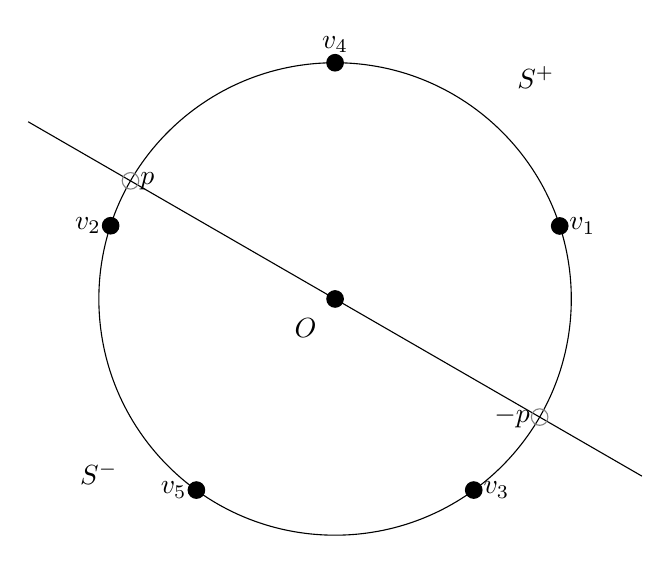
\begin{tikzpicture}[scale=1.5]

 \draw[-] (-2.598,1.5) -- (2.598,-1.5) ;
  \path (1.7,1.7) node[above]{$S^{+}$};
  \path (-2,-1.3) node[below]{$S^{-}$};
 \draw (0,0) circle (2);
 \path (-0.25,-0.25) node(axis0){$O$};
 \draw[fill, black] (0,0) circle [radius=.07cm];
 \path (-1.732,1) node(text1)[right]{$p$};
 \draw[gray] (-1.732,1) circle [radius=.07cm];
\path (1.732,-1) node(text2)[left]{$-p$};
\draw[gray] (1.732,-1) circle [radius=.07cm];
\path (0,2) node(text3)[above]{$v_4$};
\draw[fill, black] (0,2) circle [radius=.07cm];
\path (1.902,0.618) node(text4)[right]{$v_1$};
 \draw[fill, black] (1.902,0.618) circle [radius=.07cm];
 \path (-1.9,0.62) node(text4)[left]{$v_2$};
 \draw[fill, black] (-1.9,0.62) circle [radius=.07cm];
 \path (1.174,-1.618) node(text4)[right]{$v_3$};
 \draw[fill, black] (1.174,-1.618) circle [radius=.07cm];
 \path (-1.174,-1.618) node(text4)[left]{$v_5$};
 \draw[fill, black] (-1.174,-1.618) circle [radius=.07cm];
\end{tikzpicture}

\caption{This is an illustration for the proof of Lemma \ref{tech}. Here $d=5$ and $\th_1 = \frac{4\pi}{5}$. The straight line is the intersection $H_\b \cap D$.}
\end{figure}

\begin{exampleplain}
	Let $W$ be of type $B_3$ and $\Pi=\{1, 2, 3\}$ such that $\a_3$ is the unique short simple root and $s_{13} = s_{31}$. Let $w=s_{12323}$. Then $\th_1 = \pi/2$, $d = 4$ and $w = \d_1 w_1$, where $\d_1 = s_{1232}$, $w_1 = s_3$, $\Pi_1=\{3\}$ and $V^{\d_1} = \mathbb R \a_3$. As in \ref{setup}, we take $v = \a_3$. Hence $z = s_{21}$, $y = s_{23}$ and $K=\{2, 3\}$. One checks that each root of $\Delta^- - z\i(\Delta_{\Pi_1}) - \Delta_K=\{-(\a_1), -(\a_1+\a_2), -(\a_1+\a_2+2 \a_3), -(\a_1+2 \a_2+2 \a_3)\}$ appears exactly one of the sets $\{-y^i(\a_1+\a_2)\}$ for $0 \le i \le 3$.
\end{exampleplain}

\subsection{Proof of Theorem \ref{t:main}}
We argue by induction on the triple $(\Delta, \d, w)$. If $\Delta=\emptyset$, then the statement is trivial. Suppose that $\Delta \neq \emptyset$ and that the statement is true for any triple $(\Delta'', \d'', w'')$ with $|\Delta''|<|\Delta|$. Then by induction for $(\Delta_1, \d_1, w)$, $n(w)$ is conjugate to $n(\d_1) \exp(\frac{2 \pi i \phi_1^\vee}{d})$ and hence conjugate to $n(z)^{-1} n(\d_1) \exp(\frac{2 \pi i \phi_1^\vee}{d}) n(z)$.

By the computation in Section \ref{5.3}, we have $$n(z)^{-1} n(\d_1) \exp(\frac{2 \pi i \phi_1^\vee}{d}) n(z)=n(y) t \exp(\frac{2 \pi i z^{-1}(\phi_1^\vee)}{d}),$$ where
$t=\exp (\pi i\sum_{\b \in \Delta^+ \cap z(\Delta^-) \cap \d_1 \i(\Delta^-)} z^{-1}(\b^\vee))$.
By Lemma \ref{tech}, with $c=\frac{d\theta_1}{2\pi}$ we have
$$
\prod_{0 \le j \le d-1} y^j(t)=\exp(2\pi i c (\rho^\vee-z^{-1}(\rho_{\Pi_1}^\vee)-\rho_K^\vee)).
$$

For any subgroup $H$ of $G$ and $g, g' \in {}^\d G$, we write $g \sim_H g'$ if $g'=h g h \i$ for some $h \in G$.

Let $L_K$ is the standard Levi subgroup of $G$ with root system $\Delta_K$ whose derived subgroup is denoted by $G_K$. We have
\begin{align*}
  n(w) &\sim_G  n(y) t \exp(\frac{2 \pi i z^{-1}(\phi_1^\vee)}{d}) \\
       & \sim_T n(y) \exp(\frac{2\pi i c (\rho^\vee-z^{-1}(\rho_{\Pi_1}^\vee)-\rho_K^\vee)}{d}) \exp(\frac{2 \pi i z^{-1}(\phi_1^\vee)}{d}) \\
       & \sim_{G_K} \d \exp(\frac{2 \pi i c \rho_K^\vee}{d}) \exp(\frac{2\pi i c (\rho^\vee-z^{-1}(\rho_{\Pi_1}^\vee)-\rho_K^\vee)}{d}) \exp(\frac{2 \pi i z^{-1}(\phi_1^\vee)}{d}) \\
       &=\d \exp(\frac{2\pi i (c\rho^\vee + z^{-1}(\phi_1^\vee - c\rho_{\Pi_1}^\vee))}{d}) \\
       &=\d \exp(\frac{2\pi i (c\rho^\vee + \overline{\l_1^\vee})}{d})
        =\d \exp(\frac{2 \pi i \l_0^\vee}{d}).
\end{align*}
Here the second conjugation follows from Lemma \ref{average}; the third one follows from Proposition \ref{regular} and that $\rho^\vee-z^{-1}(\rho_{\Pi_1}^\vee)-\rho_K^\vee, z^{-1}(\phi_1^\vee)$ are central for $G_K$. The proof is finished.

\sec{Kac diagrams}
\label{s:kac}

We consider a connected complex semisimple group $G$, with Cartan subgroup $T$, root system $\Delta$,
simple roots $\Pi$ and Weyl group $W$. We are also given
an  automorphism $\delta$ of $G$, possibly trivial, of finite order $n$, preserving a pinning $(G,T,\{X_\alpha\mid \alpha\in\Pi\})$.
The semisimple
conjugacy classes of $G\delta$ of finite order are parametrized by their
{\it Kac diagrams}. We summarize the statements here, and refer to
\cite{ov}, \cite{kac_book} and \cite{reeder_torsion} for details.


Let $X^*$, respectively $X_*$, be the lattice of characters (resp. co-characters) of $T$.
Let $R=\Z\langle\Delta\rangle\subset X^*$ be
the root lattice, and $\ch\Delta\subset \ch R\subset X_*$ the co-roots and co-root lattice.

Recall that $V=X_*\otimes\Q$. Then $\delta$ acts on $V$, and we also write
$\delta$ for the transpose action on $V^*=\Hom_\Q(V,\Q)$.
We write $\delta$ as a superscript to denote fixed points.
We identify $(V^\delta)^*$ with $(V^*)^\delta$, and we view this as a subset of $\Lie(T)$.

We can write $T=(T^\delta)^0(1-\delta)T$, where $\phantom{}^0$ denotes identity component,
and $(1-\delta)T=\{t\delta(t\inv)\mid t\in T\}$. Both components are (connected) tori.
It follows easily from this that every element of $G\delta$ is $G$-conjugate
to an element of $(T^\delta)^0$.

Define
\begin{equation}
\label{e:e}
e(\ch\gamma)=\exp(2\pi i\ch\gamma) \quad(\ch\gamma\in V^\delta).
\end{equation}
This map is surjective  onto the elements of finite order in $(T^\delta)^0$.

Although we will make no use of this fact, it is interesting to note that if $G$ is simple then
$G^\delta$  and $T^\delta$ are connected.

Let $\Pi_\delta$ the set of orbits of $\delta$ on $\Pi$. The map
$\Pi\ni\alpha\mapsto \alpha|_{T^{\delta}}$ identifies $\Pi_\delta$ with 
a set of simple roots of 
$G^{\delta}$. Write $\Pi_\delta=\{\alpha_1,\dots,\alpha_r\}$.

Let $\Delta_\delta$ be the root system of
$(T^{\delta})^0\subset (G^{\delta})^0$, and let
$\ch\Delta_\delta=\{\ch\alpha\mid \alpha\in\Delta_\delta\}\subset
V^\delta$ be the canonical coroots defined by
(\cite{bourbaki_4-6}*{Chapter 6, Section 1.1}).
Set $\ch R_\delta=\Z\langle\ch\Delta_\delta\rangle$, the coroot lattice of $\Delta_\delta$.
Then
$$
X_*((T^{\delta})^0)=(X_*)^\delta\quad\text{and}\quad \ch R_\delta=(\ch R)^\delta.
$$

Define projection $P:V\rightarrow V^\delta$ by
$P(v)=\frac1n \sum_{i=0}^{n-1}\delta^iv$.
Then $P(X_*)$ is a lattice containing $X_*^\delta$ of finite index.
The group $W_\delta$ acts on $P(X_*)$ and $P(\ch R)$. Define:
\begin{equation}
\label{e:affine}
\begin{aligned}
\wh W_\delta&=W^\delta\ltimes P(X_*), \\
\wt W_\delta&=W^\delta\ltimes P(\ch R).
\end{aligned}
\end{equation}
Then $\wt W_\delta$ is an affine Weyl group. Let $\overline C$ be a
fundamental domain for the action of $\wt W_\delta$ on $V^\delta$.
Furthermore
$\wh W_\delta$ is an extended affine Weyl group, and
$$
\Omega=\wh W_\delta/\wt W_\delta\simeq P(X_*)/P(\ch R)
$$
is a finite group which acts naturally on $\overline C$.

\begin{lemma}
\label{l:Omega}
If $G$ is adjoint then $\Omega\simeq \pi_1(G^\delta)$.
\end{lemma}

\begin{proof}
If $\delta=1$ this is standard. In general since $G$ is adjoint it
reduces easily to the simple case and then a case-by-case check. In
fact in the twisted cases $\Omega$ is trivial except for $\twoAodd$ and $\twoD$, in which case it has order $2$.
\end{proof}



\begin{lemma}
\label{l:kac1}
Every semisimple conjugacy class of finite order in $G\delta$ is of
the form $[e(\ch\gamma)\delta]$ for some $\ch\gamma\in V^\delta$.
  
In particular suppose $\ch\gamma,\ch\tau\in V^\delta$.  Then $[e(\ch\gamma)\delta]=[e(\ch\tau)\delta]$ if and only if there exists $w\in \wh W_\delta$
such that $w\ch\gamma=\ch\tau$.

Suppose $\ch\gamma,\ch\tau\in \overline C$. Then
$[e(\ch\gamma)\delta]=[e(\ch\tau)\delta]$ if and only if there exists
$\omega\in \Omega$ such that $\omega(\ch\gamma)=\ch\tau$.

\end{lemma}

\begin{proof}[Sketch of proof]
We've already discussed the first assertion. The second follows from
the calculation that
$$
e(\ch\mu)e(\ch\gamma)\delta e(-\ch\mu)=e((1-\delta)\ch\mu+\ch\gamma)\delta\quad (\ch\mu\in V,\ch\gamma\in V^\delta)
$$
and the fact that
$$
[(1-\delta)V+X_*]^\delta=P(X_*).
$$
The final assertion is standard.
\end{proof}

We now apply the  theory of  affine Weyl groups to describe $\overline C$
when $G$ is simple.
Set $\zeta=e^{2\pi i/n}$ and let
$$
\g[\zeta]=\{X\in \g\mid \Ad(g)(X)=\zeta X\}.
$$
Then $\g[\zeta]$ is $T^\delta$ invariant. Let $\alpha_0$ be the lowest weight of $T^\delta$ acting on $\g[\zeta]$.
Then
$$
-\alpha_0=
\begin{cases}
  \text{highest root of }\Delta_\delta, &\text{ if } \delta=1;\\
  \text{highest short root of }\Delta_\delta, &\text{ if }\delta\ne 1,\Pi^\delta\ne\emptyset;\\
  \text{2*highest short root of }\Delta_\delta, &\text{ if }\delta\ne 1,\Pi^\delta=\emptyset.
\end{cases}
$$
The last case occurs if $G$ is of type $A_{2n}$ and $\delta$ has order $2$ (type $\twoAeven$).
Set $\wt\Pi_\delta=\{\alpha_0,\alpha_1,\dots,\alpha_r\}$,
and let $\ch\gamma_1,\dots,\ch\gamma_i\in V^\delta$ be the corresponding fundamental co-weights.
Define integers $c_0,c_1,\dots, c_r$ by $c_0=1$ and 
$$
\sum_{i=0}^r c_i\alpha_i=0.
$$
We define the {\it affine Dynkin diagram}  $\Daffine$ of $(G,\delta)$ to be the
Dynkin diagram of $\wt\Pi_\delta$. We equip each node with its label $c_i$.
See \cite{ov}*{Reference Chapter,Table 6} for a list of these diagrams.

The automorphism group of $\Daffine$ is isomorphic to the
automorphism group of $\overline C$. The group $P(X_*)$ acts by
translation on $V^\delta$, and this induces an action of $\Omega$ on
$\overline C$ and $\Daffine$.



Let $\wt\alpha_0$ be the affine function
$$
\wt\alpha_0=\alpha_0+\frac1n.
$$
We define the {\it affine coordinates} of  $\ch\gamma\in V^\delta$ to be
$$
(\wt\alpha_0(\ch\gamma),\alpha_1(\ch\gamma),\dots, \alpha_r(\ch\gamma)).
$$
The affine coordinates $(a_0,\dots, a_r)$ of a point  in $V^\delta$ satisfy
$\sum_{i=0}^r c_ia_i=\frac1n$.

For the fundamental domain $\overline C$ we take
points whose affine coordinates $(a_0,\dots, a_r)$ satisfy $a_i\ge 0$ $(0\le i\le r)$.


\begin{definition}
A Kac diagram for $(G,\delta)$ is a vector $\mathcal D=[a_0,\dots, a_r]$ where
each $a_i$ is a non-negative integer and $\text{GCD}(\{a_0,\dots, a_r\})=1$.
Set $d(\D)=\sum_{i=0}^r a_ic_i$, $n=\text{order}(\delta)$, and define
$$
e(\D)= e(\frac n{d(\D)}\sum_{i=1}^r a_i\ch\gamma_i)\delta.
$$
\end{definition}
Note that $\frac n{d(\D)}\sum_{i=1}^r a_i\ch\gamma_i\in \overline C$.
Here is the conclusion.


\begin{proposition}
  \label{p:kac}
Suppose $g\delta\in G\delta$ satisfies $g^d\in Z(G)$. Then there is a Kac diagram $\D$,
with $d(\D)=d$, such that $[g\delta]=[e(\D)]$.

If $\D,\mathcal E$ are Kac diagrams then $[e(\D)]=[e(\mathcal E)]$ if and only if
there exists $\omega\in \Omega$ satisfying $\omega(\D)=\mathcal E$.
\end{proposition}

We examine the role of the group $\Omega$ more closely.  If
$z\in Z(G^\delta)$ the map $[g\delta]\rightarrow [zg\delta]$ is a well
defined map of conjugacy classes in $G\delta$. Via the Proposition
this induces an action of $Z(G^\delta)$ on Kac diagrams.

Note that the Kac diagrams for $G$ are independent of isogeny; the
only role that isogeny plays is in the action of $\Omega$.  So suppose
$\D$ is a Kac diagram. View it as giving a conjugacy class of finite
order in $\Gsc\delta$ where $\Gsc$ is the simply connected cover of
$G$.  Thus $Z((\Gsc)^\delta)$ acts on Kac diagrams. Recall
$\Omega\simeq \pi_1((\Gsc)^\delta)$, which is a quotient of
$Z((\Gsc)^\delta)$.
This is compatible with Proposition \ref{p:kac}: if $z\in Z((\Gsc)^\delta)$ and $\D$ is a Kac diagram then
$$
[e(z\D)] = [p(z)e(\D)],
$$
where $p:Z((\Gsc)^\delta)\rightarrow Z(G^\delta)$. 

\begin{lemma}\label{6.7}
The orbits of  $Z((\Gsc)^\delta)$  and  $\Aut(\Daffine)$  on  the nodes of $\Daffine$
are the same.
\end{lemma}

\begin{proof}
The nodes with label $1$ are in bijection with $Z((\Gsc)^\delta)$,
so the action of $Z((\Gsc)^\delta)$ on these nodes is simply
transitive and the result is immediate.
The remaining nodes follow from a case--by--case check.
\end{proof}



\begin{proposition}
\label{p:fixed}
Suppose $w\delta\in W\delta$ is elliptic, and $n(w\delta)\in G\delta$ is a representative of $w$.
Then the Kac diagram of $n(w\delta)$ is fixed by $\Aut(\Daffine)$.
\end{proposition}

\begin{proof}
Suppose $w\delta\in W\delta$, with representative
$g\delta\in G\delta$.  If $z\in ZG^\delta$ then $zg\delta$ is also a
representative of $w\delta$, so if $w\delta$ is elliptic
then $[zg\delta]=[g\delta]$.  Therefore the Kac diagram of $[g\delta]$ is
fixed by $Z(G^\delta)$, hence by $Z((\Gsc)^\delta)$ (which acts by
projection), and hence by $\Aut(\Daffine)$ by 
Lemma \ref{6.7}.
\end{proof}


For example in (untwisted) type $A_n$ every node has label $1$, so the
only Kac diagram which is fixed by all automorphisms has all labels
$1$, which corresponds to the Coxeter element. This proves the well-known fact
that this is the the only elliptic conjugacy class in this case.


\sec{Some applications to elliptic conjugacy classes}
In this section, we make a digression and discuss some applications to elliptic conjugacy classes of finite Weyl groups. 

\begin{proposition}\label{stable-d'}
Assume that $W$ is irreducible. Then every elliptic $W$-conjugacy class of $W\delta$ is stable under the diagram automorphisms of $W$
which commute with $\delta$.
\end{proposition}

\begin{remark}
  In fact, the result is true for any finite Coxeter group (see \cite{geck_pfeiffer}*[Theorem 3.2.7] when $\d=id$ and
  \cite{he_minimal_length_double_cosets}*[Theorem 7.5] in general). The original proof (even for finite Weyl groups) is based on a characterization of elliptic conjugacy classes via the characteristic polynomials and length functions. Such characterization is established via a laborious case-by-case analysis on the elliptic conjugacy classes with the aid of computer for exceptional groups. Now we give a general proof for finite Weyl groups via the Kac diagram. 
\end{remark}

\begin{proof}
  This follows easily from Proposition \ref{p:fixed}. If $\tau$ is an
  automorphism of $W$, commuting with $\delta$, it induces an
  automorphism of $\Wext$, preserving $W\delta$. Let $G$ be the corresponding simply connected group.
  Then $\tau$ lifts to an automorphism, also denoted $\tau$, of $G$.
  If $w\delta\in W\delta$ is elliptic, so is $\tau(w\delta)$, and
  $[\tau(w\delta)]=[w\delta]$ if and only if $[\tau(n(w\delta))]=[n(w\delta)]$, where $n(w\delta)$ is a representative
  in $G\delta$ of $w\delta$, i.e. $\tau(n(w\delta))$ and $n(w\delta)$ have the same Kac diagram.
  Now the result follows from Proposition \ref{p:fixed}.
\end{proof}

The Proposition \ref{stable-d'} is used in an essential way to prove that in finite Weyl groups, elliptic conjugacy classes never fuse. 

\begin{theorem}\label{fuse}
	Let $W$ be a finite Weyl group and $\mathcal O$ be a $W$-conjugacy class of $W \d$. Let $J \subset I$ with $\d(J)=J$ and $\mathcal O \cap W_J \d$ contains an elliptic element of $W_J \d$. Then $\mathcal O \cap W_J \d$ is a single conjugacy class of $W_J$. 
\end{theorem}

This result was first proved in \cite{geck_pfeiffer}*[Theorem 3.2.11] when $\d=id$ and in
\cite{CH}*[Theorem 2.3.4] in general. The strategy is to first reduce to the case where $W$ is irreducible, then to reduce to the case where $W_J$ is irreducible. Note that the different $W_J$-conjugacy classes in $\mathcal O \cap W_J \d$ are obtained from one another by diagram automorphisms of $W_J$. The final (and crucial) step in \cite{geck_pfeiffer} and \cite{CH} was to use the characterization of elliptic conjugacy classes to deduce that the intersection is a single $W_J$-conjugacy class. Now the final step may be replaced by Proposition \ref{stable-d'}, the proof of which is simpler than the characterization of elliptic conjugacy classes. 

\sec{Non-Elliptic elements}
\label{s:nonelliptic}

For $w \in W$, we denote by $\text{supp}(w)$ the support of $w$, i.e., the set of simple reflections that occur in some (or equivalently, any) reduced expression of $w$. We define $$\text{supp}(w\delta): =\bigcup_{i \in \mathbb Z} \delta^i(\text{supp}(w)).$$ 

By \cite{geck_pfeiffer}*[\S 3.1] and
\cite{he_minimal_length_double_cosets}*[\S 7], a conjugacy class of $\Wext$ is
elliptic if and only if it does not intersect with
${}^\delta W_J=W_J \rtimes \langle \delta \rangle$ for any proper
$\delta$-stable subsets $J$ of $\Pi$, in other words,
$\text{supp}(w)=\Pi$ for any $w$ in the conjugacy class.

We have the following result (see \cite{geck_pfeiffer}*[Corollary
3.1.11] for untwisted conjugacy classes and \cite{CH}[Proposition
2.4.1] in the general case).

\begin{proposition}\label{x-delta}
	Let $w_1, w_2 \in W\delta$ be minimal length elements in the same conjugacy class. Let $J_i=\text{supp}(w_i)$ for $i=1,2$. Then there exists $x \in {}^{J_2} W^{J_1} \cap W^\delta$ with $x J_1 x^{-1}=J_2$. 
\end{proposition}

Consider the set $\mathcal P_{\delta}$ of pairs $(J, D)$, where $J \subset \Pi$ is a $\delta$-stable subset and $D \subset W_J \delta$ is an elliptic conjugacy class of ${}^\delta W_J$. The equivalence relation on $\mathcal P_{\delta}$ is defined by $(J, D) \sim (J', D')$ if there exists $x \in {}^{J'} W^J \cap W^\delta$ such that $x J x^{-1}=J'$ and $x D x^{-1}=D'$. 

Combining Theorem \ref{fuse} with Proposition \ref{x-delta}, we have 

\begin{theorem}\label{cal-P}
	The map $$C \mapsto \{(J, C \cap W_J \delta); J=\text{supp}(w) \text{ for some } w \text{ of minimal length in } C\}$$ induces a bijection from $[W\delta] \to \mathcal P_{\delta}/\sim$. 
\end{theorem}

For untwisted conjugacy classes, the statement is obtained by Geck and
Pfeiffer in \cite{geck_pfeiffer}*[Theorem 3.2.12]. The general case is
proved in a similar way.

Let $C\in [\Wext]$ and $w \in C$. In general the lifts of $w$ to $\Gext$ are not $G$-conjugate. However there is a reasonable canonical choice of this lifting, defined as follows.

Without loss of generality, we assume that $C \subset W \delta$. Let $(J, D) \in \mathcal P_{\delta}$ be an element corresponds to $C$. Let $L_J$ be the standard Levi subgroup corresponds to $J$.  Apply the algorithm of Section \ref{const} to $({}^\delta L_J, D)$ to construct a conjugacy class $\Psi_J(D)$ in ${}^\delta L_J$, and thus (by acting by $G$) a conjugacy class $\widetilde{\Psi_J(D)}$ in $\Gext$.

\begin{proposition} The map $$[W \delta] \to [\Gext^{\ss}], \qquad C \mapsto \widetilde{\Psi_J(D)}$$ is well-defined. 
\end{proposition}

\begin{proof}
	Let $(J, D), (J', D')$ be elements in $\mathcal P_{\delta}$ that correspond to $C$. By Theorem \ref{cal-P}, there exists $x \in {}^{J_2} W^{J_1} \cap W^\delta$ with $x J_1 x^{-1}=J_2$. As discussed in \cite{AH}*{Section 2} the Tits group provides a section $\sigma:W\rightarrow \Norm_G(T)$ satisfying
	$\delta(\sigma(w))=\sigma(\delta(w))$. In particular, $\sigma(x)$ is $\delta$-stable. Since $x J x^{-1}=J'$, we have $\sigma(x) L_J \delta(\sigma(x))^{-1}=\sigma(x) L_J \sigma(x)^{-1}=L_{J'}$. Since $x D x^{-1}=D'$, we have $\sigma(x) \Psi_J(D) \sigma(x)^{-1}=\Psi_{J'}(D')$. Hence $\widetilde{\Psi_J(D)}=\widetilde{\Psi_{J'}(D')}$. 
\end{proof}

\sec{Tables}
\label{s:tables}

For each exceptional group we list representatives of the elliptic conjugacy classes in $W$,
their Kac diagrams, and some other information.

We use the Bourbaki numbering of the simple roots \cite{bourbaki_4-6}.
Each table is preceded by the affine Dynkin diagram with the labels of the nodes.


\begin{enumerate}
\item Name: name of the elliptic conjugacy class, as in \cite{carter_conjugacy_classes} and \cite{geck_pfeiffer}.
\item d: order of the elements in the conjugacy classes.
\item Kac diagram: with respect to the given affine Dynkin diagram.
\item Centralizer: type of the derived group of the centralizer.
\item good: $w^d$ in the braid monoid (see Theorem \ref{t:braid}).
\item description: Realizing $w$ as the power of the Coxeter element of $G$ or a subgroup;
  the long element $w_0$;
if $w$ is regular (r).
\end{enumerate}

In many cases one can use a combination of techniques to compute Kac
coordinates.  If $w$ is contained in the Weyl group of a proper subgroup
then its Kac coordinates can
be calculated in this subgroup. 
Also if  $w$ is $d$-regular then $[t(w)]=\e(\ch\rho/d)\delta$, see Section
\ref{s:regular} and \cite{reeder_torsion}*{Section 2.6}.  
One needs to use the affine Weyl group to move $\ch\rho/d$ to the
fundamental alcove to compute the Kac coordinates.

Suppose $w$ is an elliptic element, and 
$[n(w)]=[\e(\ch\gamma)\delta]$. In some cases powers of $w$ are also elliptic. If  $w^k$ is also elliptic then
$[n(w^k)]=[\e(k\ch\gamma)\delta]$.  Thus the Kac coordinates are
those of the image of $k\ch\gamma$ in the fundamental alcove under the
affine Weyl group. Again there is no closed formula for these
coordinates.

There are very few elliptic conjugacy classes not amenable to these methods.
For example in $E_8$ the only cases not handled this way are 
$E_8(a4)$ and $E_8(a7)$. 

\begin{exampleplain}
Consider the conjugacy class $E_8(a_7)$ of  $W(E_8)$
\cite{geck_pfeiffer}*{Table B.6}. We take the following
representative
$$
w=2343654231435426543178
$$
of order $d=12$ and length $22$. Let $\zeta$ be a primitive $12^{th}$ root of unity.
The eigenvalues of $w$ are $\{\zeta^k\mid k=1,2,5,7,10,11\}$.
The dimension of the eigenspaces are $1,2,1,1,2,1$, respectively.
In the notation of the algorithm we have
$$
\Gamma_w=\{\theta_1,\theta_2,\theta_3\}=\{2\pi /12, 4\pi /12, 10\pi /12\}=\frac{2\p}{12}*\{1,2,5\}.
$$
Note that
$$
\frac{d(\theta_2-\theta_1)}{2\pi}=\frac{d(\theta_1-\theta_0)}{2\pi}=1.
$$
We have
$$
0=F_0\subset F_1\subset F_2\subset F_3=V,
$$
where the $F_i$ have dimensions $0,2,6$ and $8$, respectively.

In particular $F_1=V(w,2\pi/12)$ is two-dimensional.  The set $\Delta_1$ of roots vanishing on this space
is a standard Levi subgroup of type $D_4$, with simple roots $\{2,3,4,5\}$.
It turns out that $\Delta_2=\emptyset$, so we have

  $$
  \Delta=\Delta_0=E_8\supset \Delta_1=D_4\supset \Delta_2=\Delta_3=\emptyset.
$$

The algorithm gives the following elements in turn:
$$
\ch\lambda_3=\ch\lambda_2=0,
$$
$$
\ch\lambda_1=\frac{d(\theta_2-\theta_1)}{2\pi}\ch\rho_1=\ch\rho_1.
$$
Next find $w\in W(\Delta_0)=W$ so that $w\ch\rho_1$ is dominant, and then set
$$
\ch\lambda_0=\frac{d(\theta_1-\theta_0)}{2\pi}\ch\rho+w\ch\rho_1=\ch\rho+w\ch\rho_1.
$$
In fundamental weight coordinates we have
$$
\begin{aligned}
  \ch\rho_1&=(-3,1,1,1,1,-3,0,0),\\
  w\ch\rho_1&=(0,0,0,0,0,0,1,1),\\
  \ch\lambda_0=\ch\rho+w\ch\rho_1&=  ( 1,1,1,1,1,1,2,2),\\
  \ch\lambda_0/12&=(  1,1,1,1,1,1,2,2)/12.
\end{aligned}
$$
This element is dominant but not in the fundamental alcove; its affine coordinates are
$$
(1,1,1,1,1,1,2,2,-22)/12.
$$
Applying the affine Weyl group takes this to the element $(0,0,1,0,1,0,0,1)/12$,
or affine coordinates  $(0,0,1,0,1,0,0,1,1)/12$. The corresponding  Kac coordinates are therefore $(0,0,1,0,1,0,0,1,1)$.
Note that the sum of the coefficients times the corresponding labels is $1*4+1*5+1*2+1*1=12$.
See the corresponding line in the $E_8$ table. 
Compare \cite{rgly}*{Section 8}.
\end{exampleplain}

\begin{remarkplain}
In \cite{geck_pfeiffer}*{Table B.6} there is a different
representative for this conjugacy class.
Although this representative is good,
it turns out the positive chamber is not in good position for this element
(both ``good'' and ``good position'' are defined in Section \ref{s:digression}), and
in particular the Levi subgroups defined by \eqref{e:levis} are not standard.
\end{remarkplain}
\bigskip


$$
G_2:\quad \begin{dynkinDiagram}[Kac,extended,root radius=.12cm, edge length=1.0cm]{G}{2}
\dynkinLabelRoots{1,2,3}
\end{dynkinDiagram}
$$

\begin{tabular}{|l|l|l|l|l|l|l|l|}
\hline
w&   d    &  Kac diagram &good&Centralizer&description\\\hline
$12$ & $6$ &   $111$ & $\Delta^2$&$*$ & Cox,r\\\hline
$1212$ & $3$ &  $110$ & $\Delta^2$&$A_1$ &Cox$^2,r$\\\hline
$w_0$ & $2$ &  $010$ & $\Delta^2$&$2A_1$ & Cox$^6,r$\\\hline
  \end{tabular}

  \bigskip

$$
^3D_4:\quad \begin{dynkinDiagram}[Kac,extended,root radius=.12cm, edge length=1.0cm]{D}[3]{4}
\dynkinLabelRoots{1,2,1}
\end{dynkinDiagram}
$$

\begin{tabular}{|l|l|l|l|l|l|l|l|}
\hline
w&   d    &  Kac diagram &good&Centralizer&description\\\hline
  $12$ & $12$ &   $111$ & $\Delta^2$&$*$ &Cox,r\\\hline
  $132132$ & $6$ &   $010$ & $\Delta^2\Delta_{23}^4$&$2A_1$ &\\\hline
  $1323$ & $6$ &   $101$ & $\Delta^2$&$A_1$ &r\\\hline
      $13213423$ & $3$ &   $001$ & $\Delta^2$&$A_2$ &Cox$^4$,r\\\hline
  \end{tabular}

\newpage

  

$$
F_4:\quad \begin{dynkinDiagram}[Kac,extended,root radius=.12cm, edge length=1.0cm]{F}{4}
\dynkinLabelRoots{1,2,3,4,2}
\end{dynkinDiagram}
$$

\medskip
\setlength\extrarowheight{3pt}

\begin{tabular}{|l|l|l|l|l|l|}
\hline
Name&   d    &  Kac diagram &good&Centralizer&description\\\hline
$F_4$ & $12$ &   $11111$ & $\Delta^2$&$*$ & $\cox(F_4)$,r\\\hline
$B_4$ & $8$ &   $11101$ & $\Delta^2$&$A_1$ &r\\\hline
$F_4(a1)$ & $6$ &  $10101$ & $\Delta^2$&$2A_1$ &r\\\hline
$D_4$ & $6$ &  $11100$ & $\Delta^2\Delta_{34}^4$&$A_2$ &\\\hline

$C_3+A_1$ & $6$ &   $01010$ & $\Delta^2\Delta_{12}^4$&$3A_1$ &\\\hline
$D_4(a1)$ & $4$ &   $10100$ & $\Delta^2$&$A_1+A_2$ &r\\\hline
$A_3+\wt A_1$ & $4(8)$ &   $02010$ & $\Delta^2\Delta_{23}^2$&$3A_1$ &\\\hline
$A_2+\wt A_2$ & $3$ &   $00100$ & $\Delta^2$&$2A_2$ &r\\\hline
$4A_1$ & $2$ &   $01000$ & $\Delta^2$&$A_1+C_3$ &$w_0$,r\\\hline
\end{tabular}

\medskip

The conjugacy class $A_3+\wt A_1$ of $W$ has order $4$, but its lift
to a semisimple conjugacy class has order $8$ \cite{AH}*{Theorem B}.

\bigskip



$$
^2E_6:\quad \begin{dynkinDiagram}[Kac,extended,root radius=.12cm, edge length=1.0cm]{E}[2]{6}
\dynkinLabelRoots{1,2,3,2,1}
\end{dynkinDiagram}
$$

\medskip
\setlength\extrarowheight{5pt}
\hskip-.5in
\begin{tabular}{|l|l|l|l|l|l|l|l|}
\hline
  w&   d    &  Kac diagram &good&Centralizer&description\\\hline
$1254$                            &  18  &  $11111$   & $\Delta^2$&*&$\cox(^2E_6)$,r\\\hline
$123143$                  &  12  &  $11011$   &$\Delta^2$&$A_1$&r\\\hline
  $45423145$                   &  10  &  $01011$  &  $\Delta^2\Delta_4^8$&$2A_1$&\\\hline
$1231431543165431$   &  $6$ & $ 1 1 0 0 0$   &$\Delta^2\Delta_{1356}^4$&$B_3$& \\\hline
  $425423456542345$   &  6   &  $00100$    &$\Delta^2\Delta_{2345}^2$&$2A_2$&\\\hline
  $23423465423456$   &  6    &    $00011$     & $\Delta^2\Delta_{24}^4$&$A_3$&\\\hline
  $124315436543$   & $6$ & $01001$ &$\Delta^2$ & $A_1+B_2$ &r \\\hline
$142314354231365431$ &  4  &  $00010$   &$\Delta^2$&$A_1+A_3$&r\\\hline
  $w_0$     & $2$ &   $00001$ & $\Delta^2$&$C_4$ &r \\\hline
\end{tabular}

\newpage

$$
E_6:\quad \begin{dynkinDiagram}[Kac,extended,root radius=.12cm, edge length=1.0cm]{E}{6}
\dynkinLabelRoots{1,1,2,3,2,1,2}
\end{dynkinDiagram}
$$

\medskip

\begin{tabular}{|l|l|l|l|l|l|l|}
  \hline
  Name&   d &  Kac diagram &good&Centralizer&description\\\hline
      &         &      $\phantom{11}1$&&&\\
      &         &      $\phantom{11}1$&&&\\
  $E_6$ & $12$ &   $11111$ & $\Delta^2$&$*$ & $\cox(E_6)$,r\\\hline
        &          &      $\phantom{11}1$&&&\\
      &         &      $\phantom{11}1$&&&\\
  $E_6(a1)$ & $9$ &   $11011$ & $\Delta^2$&$A_1$ &r\\\hline
        &         &      $\phantom{11}1$&&&\\
      &         &      $\phantom{11}0$&&&\\
  $E_6(a2)$ & $6$ &  $10101$ & $\Delta^2$&$3A_1$ &r\\\hline
             &  &      $\phantom{11}0$&&&\\
&           &          $\phantom{11}1$&&&\\
  $A_5+A_1$ & $6$ &  $01010$ & $\Delta^2\Delta_{24}^4$&$4A_1$ &\\\hline
            &  &      $\phantom{11}0$&&&\\
 &          &          $\phantom{11}0$&&&\\
  $3A_2$ & $3$ &   $00100$ & $\Delta^2$&$3A_2$ &r \\\hline
\end{tabular}

\newpage

$$
E_7:\quad \begin{dynkinDiagram}[Kac,extended,root radius=.12cm, edge length=1.0cm]{E}{7}
\dynkinLabelRoots{1,2,3,4,3,2,1,2}
\end{dynkinDiagram}
$$

\medskip
\setlength\extrarowheight{5pt}
\begin{tabular}{|l|l|l|l|l|l|}
\hline
  Name&   d &  Kac diagram &good&Centralizer&description\\\hline
        &          &      $\phantom{111}1$&&&\\
  $E_7$     & $18$ &  $1111111$ & $\Delta^2$&$*$ & $\cox(E_7)$,r\\\hline
          &         &      $\phantom{111}1$&&&\\
  $E_7(a1)$ & $14$ &  $1110111$ & $\Delta^2$&$A_1$&\\\hline
                &    &      $\phantom{111}1$&&&\\
  $E_7(a2)$ & $12$ &  $1101011$ & $\Delta^2\Delta_{257}^2$&$2A1$ &\\\hline
      &      &          $\phantom{111}1$&&&\\
  $E_7(a3)$ & $30$ &   $3212123$ & $\Delta^2\Delta_{24}^4$&$*$ &\\\hline
        &      &          $\phantom{111}1$&&&\\
  $D_6+A_1$ & $10$ &  $0101010$ & $\Delta^2\Delta_{24}^8$&$4A_1$ &\\\hline
        &      &         $\phantom{111}0$&&&\\
  $A_7 $     & $8$ &  $0101010$ & $\Delta^2\Delta_{257}^2\Delta_{2}^4$&$2A_1+A_2$ &\\\hline
        &      &          $\phantom{111}0$&&&\\
  $E_7(a4)$ & $6$ &   $1001001$ & $\Delta^2$&$2A_2+A_1$ &\\\hline
        &      &         $\phantom{111}1$&&&\\
  $D_6(a2)+A_1$ & $6$ &  $0100010$ & $\Delta^2\Delta_{13}^4$&$2A_1+A_3$ &\\\hline
        &      &        $\phantom{111}0$&&&\\
  $A_5+A_2$  & $6$ &   $0010100$ & $\Delta^2\Delta_{2345}^2$&$3A_2$ &\\\hline
        &      &         $\phantom{111}1$&&&\\
  $D_4+3A_1$ & $6$ &   $0001000$ & $\Delta^2\Delta_{24567}^4$&$2A_3$ &\\\hline
        &      &          $\phantom{111}0$&&&\\
  $2A_3+A_1$ & $4$ &  $0001000$ & $\Delta^2\Delta_{257}^2$&$2A_3+A_1$ &\\\hline
        &      &         $\phantom{111}1$&&&\\
  $7A_1$     & $2$ &  $00000000$ & $\Delta^2$&$A_7$ &$w_0$\\\hline
\end{tabular}

\newpage
$$
E_8:\quad \begin{dynkinDiagram}[Kac,extended,root radius=.12cm, edge length=1.0cm]{E}{8}
\dynkinLabelRoots{1,2,3,4,5,6,4,2,3}
\end{dynkinDiagram}
$$

\medskip

\hskip-.4in
\begin{tabular}{|l|l|l|l|l|l|l|l|}
\hline
Name&   d &  Kac diagram &good&Centralizer&description\\\hline
        &      &          $\phantom{11}1$&&&\\
  $E_8$ & $30$ &  $11111111$ & $\Delta^2$&$*$ & $\cox(E_8)$,r\\\hline
        &      &          $\phantom{11}0$&&&\\
  $D_8(a2)$ & $30$   & $12102030$ &$\Delta^6\Delta_{2456}^4\Delta_5^{20}$ &$4A_1$ & \\\hline
        &      &          $\phantom{11}1$&&&\\
$E_8(a1)$ & $24$  &  $11011111$ & $\Delta^2$ &$A_1$ & r\\\hline
        &      &          $\phantom{11}1$&&&\\
$E_8(a2)$ & $20$  & $11010111$ & $\Delta^2$ & $2A_1$ & r\\\hline
        &      &          $\phantom{11}0$&&&\\
$E_7A_1$ & $18$  & $11101010$ & $\Delta^2\Delta_{24}^{16}$ & $4A_1$ & $\cox(E_7A_1)$\\\hline
        &      &          $\phantom{11}1$&&&\\
$E_8(a4)$ & $18$  & $01010111$ & $\Delta^2\Delta_{24}^4$ & $3A_1$ & \\\hline
        &      &          $\phantom{11}0$&&&\\
$E_8(a5)$ & $15$  &  $10101011$ & $\Delta^2$ & $4A_1$ & r\\\hline
        &      &          $\phantom{11}0$&&&\\
$D_8$ & $14$ & $10101010$ & $\Delta^2\Delta_{2}^{12}$ & $5A_1$ & $\cox(D_8)$\\\hline
        &      &          $\phantom{11}0$&&&\\
$E_8(a3)$ & $12$  &$10100101$ & $\Delta^2$ & $3A_1+A_2$ & r\\\hline
        &      &          $\phantom{11}0$&&&\\
$E_8(a7)$ & $12$ & $01010011$ & $\Delta^2\Delta_{2345}^{2}$ & $A_1+2A_2$ & \\\hline
        &      &          $\phantom{11}1$&&&\\
$E_6+A_2$ & $12$ &  $00100100$ & $\Delta^2\Delta_{2345}^{6}$ & $3A_2$ & $\cox(E_6A_2)$\\\hline
        &      &          $\phantom{11}0$&&&\\
$D_5(a1)+A_3$ & $12$ & $01002000$ & $\Delta^2\Delta_{123456}^{2}$ & $3A_1+A_3$ & \\\hline
        &      &          $\phantom{11}0$&&&\\
$D_8(a1)$ & $12$ & $00101010$ & $\Delta^2\Delta_{4578}^{4}$ & $4A_1+A_2$ & \\\hline



\end{tabular}

\pagestyle{headings}
\hskip-.8in
\begin{tabular}{|l|l|l|l|l|l|l|l|}
\hline
  Name&   d&  Kac diagram &good&Centralizer&description\\\hline
          &      &          $\phantom{11}0$&&&\\
$E_7(a2)+A_1$ & $12$  &$11001010$ & $\Delta^2\Delta_{2345}^{2}\Delta_{24}^{8}$ & $2A_1+A_3$ & \\\hline
          &      &          $\phantom{11}0$&&&\\
$E_8(a6)$ & $10$  &$00100101$ & $\Delta^2$ & $2A_1+2A_2$ & $\cox(E_8)^3$,  r\\\hline
          &      &          $\phantom{11}0$&&&\\
$D_6+2A_1$ & $10$  &$11001000$ & $\Delta^2\Delta_{2456}^{8}$ & $2A_3$ & \\\hline
          &      &          $\phantom{11}0$&&&\\
$A_8$ & $9$  &$00100100$ & $\Delta^2\Delta_{34}^{4}$ & $A_1+3A_2$ & $A_8$\\\hline
        &      &          $\phantom{11}0$&&&\\
$A_1+A_7$ & $8$  &$01001000$ & $\Delta^2\Delta_{2345}^{2}\Delta_{25}^{4}$ & $A_1+2A_3$ & $\cox(A_1+A_7),\cox(A_3+D_5)$\\\hline
        &      &          $\phantom{11}0$&&&\\
$D_8(a3)$ & $8$  &$00100010$ & $\Delta^2$ & $2A_1+2A_3$ &r\\\hline
        &      &          $\phantom{11}0$&&&\\
$E_8(a8)$ & $6$  &$00010001$ & $\Delta^2$ & $A_3+A_4$ &  $\cox(E_8)^5$,  r\\\hline

        &      &          $\phantom{11}0$&&&\\
$E_7(a4)+A_1$ & $6$  &$01000010$ & $\Delta^2\Delta_{34}^{4}$ & $2A_1+A_5$ & \\\hline
        &      &          $\phantom{11}1$&&&\\
$E_6(a2)+A_2$ & $6$  &$00000100$ & $\Delta^2\Delta_{2345}^{2}$ & $A_2+A_5$ & \\\hline
        &      &          $\phantom{11}0$&&&\\
$2D_4$ & $6$  &$10001000$ & $\Delta^2\Delta_{1367}^{4}$ & $A_3+D_4$ & $\cox(2D_4)$\\\hline
        &      &          $\phantom{11}0$&&&\\
$D_4+4A_1$ & $6$  &$11000000$ & $\Delta^2\Delta_{123456}^{4}$ & $A_7$ & $\cox(D_4+4A_1)$\\\hline
        &      &          $\phantom{11}0$&&&\\
$A_1+A_2+A_5$ & $6$  &$00100000$ & $\Delta^2\Delta_{234578}^{2}\Delta_{78}^{2}$ & $A_1+A_2+A_5$ & $\cox(A_1+A_2+A_5)$\\\hline
        &      &          $\phantom{11}0$&&&\\
$2A_4$ & $5$  &$00010000$ & $\Delta^2$ & $2A_4$ & $\cox(2A_4)$,$\cox(E_8)^6,r$\\\hline
        &      &          $\phantom{11}0$&&&\\
$2A_3+2A_1$ &  $4$ &$01000000$ & $\Delta^2\Delta_{2345}^{2}$ & $A_1+A_7$ & $\cox(2A_3+2A_1)$\\\hline
        &      &          $\phantom{11}0$&&&\\
$2D_4(a1)$ & $4$  & $00001000$ & $\Delta^2$ & $A_3+D_5$ &r \\\hline
        &      &          $\phantom{11}1$&&&\\
$4A_2$ & $3$  &$00000000$ & $\Delta^2$ & $A_8$ & $\cox(4A_2)$,$\cox(E_8)^{10}$, r\\\hline
        &      &          $\phantom{11}0$&&&\\  
$8A_1$ & $2$ &$10000000$ & $\Delta^2$ & $D8$ & $\cox(8A_1)$,$\cox(E_8)^{15}$,$w_0$, r\\\hline
\end{tabular}

\bibliographystyle{plain}
%\bibliography{./refs.bib}
% \bib, bibdiv, biblist are defined by the amsrefs package.
\begin{bibdiv}
\begin{biblist}

\bib{atlas_software}{article}{
       title={Atlas of lie groups and representations software package},
        date={2019},
        note={www.liegroups.org},
}

\bib{AH}{article}{
      author={Adams, Jeffrey},
      author={He, Xuhua},
       title={Lifting of elements of {W}eyl groups},
        date={2017},
        ISSN={0021-8693},
     journal={J. Algebra},
      volume={485},
       pages={142\ndash 165},
         url={http://dx.doi.org/10.1016/j.jalgebra.2017.04.018},
      review={\MR{3659328}},
}

\bib{bourbaki_4-6}{book}{
      author={Bourbaki, Nicolas},
       title={Lie groups and {L}ie algebras. {C}hapters 4--6},
      series={Elements of Mathematics (Berlin)},
   publisher={Springer-Verlag, Berlin},
        date={2002},
        ISBN={3-540-42650-7},
         url={https://doi.org/10.1007/978-3-540-89394-3},
        note={Translated from the 1968 French original by Andrew Pressley},
      review={\MR{1890629}},
}

\bib{bouwknegt}{article}{
      author={Bouwknegt, Peter},
       title={Lie algebra automorphisms, the {W}eyl group, and tables of shift
  vectors},
        date={1989},
        ISSN={0022-2488},
     journal={J. Math. Phys.},
      volume={30},
      number={3},
       pages={571\ndash 584},
         url={https://doi-org.proxy-um.researchport.umd.edu/10.1063/1.528422},
      review={\MR{984692}},
}

\bib{carter_conjugacy_classes}{article}{
      author={Carter, R.~W.},
       title={Conjugacy classes in the {W}eyl group},
        date={1972},
        ISSN={0010-437X},
     journal={Compositio Math.},
      volume={25},
       pages={1\ndash 59},
      review={\MR{0318337}},
}

\bib{CH}{article}{
      author={Ciubotaru, Dan},
      author={He, Xuhua},
       title={The cocenter of the graded affine {H}ecke algebra and the density
  theorem},
        date={2016},
        ISSN={0022-4049},
     journal={J. Pure Appl. Algebra},
      volume={220},
      number={1},
       pages={382\ndash 410},
  url={https://doi-org.proxy-um.researchport.umd.edu/10.1016/j.jpaa.2015.06.018},
      review={\MR{3393467}},
}

\bib{gkp}{article}{
      author={Geck, Meinolf},
      author={Kim, Sungsoon},
      author={Pfeiffer, G\"{o}tz},
       title={Minimal length elements in twisted conjugacy classes of finite
  {C}oxeter groups},
        date={2000},
        ISSN={0021-8693},
     journal={J. Algebra},
      volume={229},
      number={2},
       pages={570\ndash 600},
  url={https://doi-org.proxy-um.researchport.umd.edu/10.1006/jabr.1999.8253},
      review={\MR{1769289}},
}

\bib{geck_michel_good}{article}{
      author={Geck, Meinolf},
      author={Michel, Jean},
       title={``{G}ood'' elements of finite {C}oxeter groups and
  representations of {I}wahori-{H}ecke algebras},
        date={1997},
        ISSN={0024-6115},
     journal={Proc. London Math. Soc. (3)},
      volume={74},
      number={2},
       pages={275\ndash 305},
  url={https://doi-org.proxy-um.researchport.umd.edu/10.1112/S0024611597000105},
      review={\MR{1425324}},
}

\bib{geck_pfeiffer}{book}{
      author={Geck, Meinolf},
      author={Pfeiffer, G\"otz},
       title={Characters of finite {C}oxeter groups and {I}wahori-{H}ecke
  algebras},
      series={London Mathematical Society Monographs. New Series},
   publisher={The Clarendon Press, Oxford University Press, New York},
        date={2000},
      volume={21},
        ISBN={0-19-850250-8},
      review={\MR{1778802}},
}

\bib{rgly}{article}{
      author={Gross, Benedict~H.},
      author={Levy, Paul},
      author={Reeder, Mark},
      author={Yu, Jiu-Kang},
       title={Gradings of positive rank on simple {L}ie algebras},
        date={2012},
        ISSN={1083-4362},
     journal={Transform. Groups},
      volume={17},
      number={4},
       pages={1123\ndash 1190},
  url={https://doi-org.proxy-um.researchport.umd.edu/10.1007/s00031-012-9196-3},
      review={\MR{3000483}},
}

\bib{he_minimal_length_double_cosets}{article}{
      author={He, Xuhua},
       title={Minimal length elements in some double cosets of {C}oxeter
  groups},
        date={2007},
        ISSN={0001-8708},
     journal={Adv. Math.},
      volume={215},
      number={2},
       pages={469\ndash 503},
  url={https://doi-org.proxy-um.researchport.umd.edu/10.1016/j.aim.2007.04.005},
      review={\MR{2355597}},
}

\bib{he_nie_minimal_finite}{article}{
      author={He, Xuhua},
      author={Nie, Sian},
       title={Minimal length elements of finite {C}oxeter groups},
        date={2012},
        ISSN={0012-7094},
     journal={Duke Math. J.},
      volume={161},
      number={15},
       pages={2945\ndash 2967},
  url={https://doi-org.proxy-um.researchport.umd.edu/10.1215/00127094-1902382},
      review={\MR{2999317}},
}

\bib{kac_book}{book}{
      author={Kac, Victor~G.},
       title={Infinite-dimensional {L}ie algebras},
     edition={Third},
   publisher={Cambridge University Press, Cambridge},
        date={1990},
        ISBN={0-521-37215-1; 0-521-46693-8},
  url={https://doi-org.proxy-um.researchport.umd.edu/10.1017/CBO9780511626234},
      review={\MR{1104219}},
}

\bib{ls}{article}{
      author={Langlands, R.~P.},
      author={Shelstad, D.},
       title={On the definition of transfer factors},
        date={1987},
        ISSN={0025-5831},
     journal={Math. Ann.},
      volume={278},
      number={1-4},
       pages={219\ndash 271},
      review={\MR{MR909227 (89c:11172)}},
}

\bib{ov}{book}{
      author={Onishchik, A.~L.},
      author={Vinberg, {\`E}.~B.},
       title={Lie groups and algebraic groups},
      series={Springer Series in Soviet Mathematics},
   publisher={Springer-Verlag},
     address={Berlin},
        date={1990},
        ISBN={3-540-50614-4},
        note={Translated from the Russian and with a preface by D. A. Leites},
      review={\MR{91g:22001}},
}

\bib{panyushev}{article}{
      author={Panyushev, Dmitri~I.},
       title={On invariant theory of {$\theta$}-groups},
        date={2005},
        ISSN={0021-8693},
     journal={J. Algebra},
      volume={283},
      number={2},
       pages={655\ndash 670},
  url={https://doi-org.proxy-um.researchport.umd.edu/10.1016/j.jalgebra.2004.03.032},
      review={\MR{2111215}},
}

\bib{reeder_torsion}{article}{
      author={Reeder, Mark},
       title={Torsion automorphisms of simple {L}ie algebras},
        date={2010},
        ISSN={0013-8584},
     journal={Enseign. Math. (2)},
      volume={56},
      number={1-2},
       pages={3\ndash 47},
  url={https://doi-org.proxy-um.researchport.umd.edu/10.4171/LEM/56-1-1},
      review={\MR{2674853}},
}

\bib{springer_regular}{article}{
      author={Springer, T.~A.},
       title={Regular elements of finite reflection groups},
        date={1974},
        ISSN={0020-9910},
     journal={Invent. Math.},
      volume={25},
       pages={159\ndash 198},
  url={https://doi-org.proxy-um.researchport.umd.edu/10.1007/BF01390173},
      review={\MR{0354894}},
}

\end{biblist}
\end{bibdiv}

\end{document}